\PassOptionsToPackage{english, main=french}{babel}
\documentclass[letterpaper, twoside, 12pt,%
 memoire, french, creativecommons, hyperref, withAlgo2e%
]{thETS}

\usepackage{textcomp} % Correct display of characters such as \degree
\usepackage{csquotes} % Quotations
\usepackage[binary-units=true, locale=FR]{siunitx} % Correct display of units
\usepackage{pdfpages} % Include PDFs
\usepackage{color} % Declare colors
\usepackage{inconsolata} % Better typewriter font
\usepackage{tikz-uml} % UML diagrams
\usepackage{xfrac}

% Quotations configuration
\let\oldforeignlanguage\foreignlanguage
\renewcommand{\foreignlanguage}[2]{\oldforeignlanguage{#1}{\emph{#2}}}

\babeltags{en = english}

% Refs
\newcommand{\autorefp}[2][]{(\textit{Voir} \autoref{#2}#1)}

% Figure with ÉTS style
\newcommand{\figureLayoutETS}[3]{%
  \begin{figure}%
    \centering%
    \fbox{#2}\\%
    \parbox{0.9\textwidth}{%
      \caption{#3}%
      \label{fig:#1}%
    }%
  \end{figure}%
}
\newcommand{\figureETS}[3][0.75]{%
  \figureLayoutETS{#2}{%
    \includegraphics[width=#1\textwidth]{Figures/#2}%
  }{#3}%
}
\newcommand{\subfigureETS}[3][0.25]{%
  \subfloat[#3]{%
    \includegraphics[height=#1\textheight]{Figures/#2}%
    \label{fig:#2}%
  }%
}
\newcommand{\figurehspace}[1][1]{\hspace{#1\fboxsep}}

\setcounter{lofdepth}{2} % Display subfigures in list of figures

\newcommand{\reffigureETS}[1]{\autoref{fig:#1}}
\newcommand{\reffigureETSp}[2][]{\autorefp[#1]{fig:#2}}

% Table with ÉTS style
\newenvironment{tableETS}[2]{%
  \begin{table}%
  \parbox{0.9\textwidth}{%
    \caption{#2}%
    \label{#1}%
  }%
  \centering%
}{%
  \end{table}%
}

% Vertically centered columns, based on https://tex.stackexchange.com/a/12712
\newcolumntype{L}[1]{>{\raggedright\let\newline\\\arraybackslash\hspace{0pt}}m{#1}}
\newcolumntype{C}[1]{>{\centering\let\newline\\\arraybackslash\hspace{0pt}}m{#1}}
\newcolumntype{R}[1]{>{\raggedleft\let\newline\\\arraybackslash\hspace{0pt}}m{#1}}

% Units
\DeclareSIUnit\fps{FPS}
\DeclareSIUnit\inch{pouces}
\DeclareSIUnit\px{px}
\DeclareSIUnit[per-mode=symbol]\ppd{\px\per\degree}

% Listings
\lstloadlanguages{C++, [Sharp]C, XML}

\definecolor{black}{rgb}{0,0,0}
\definecolor{blue}{rgb}{0.13,0.13,1}
\definecolor{cyan}{rgb}{0.17,0.57,0.69}
\definecolor{green}{rgb}{0,0.5,0}
\definecolor{maroon}{rgb}{0.6,0,0}
\definecolor{red}{rgb}{0.9,0,0}

% Based on https://en.wikibooks.org/wiki/LaTeX/Source_Code_Listings#Encoding_issue
\lstset{literate=
  {á}{{\'a}}1 {é}{{\'e}}1 {í}{{\'i}}1 {ó}{{\'o}}1 {ú}{{\'u}}1
  {Á}{{\'A}}1 {É}{{\'E}}1 {Í}{{\'I}}1 {Ó}{{\'O}}1 {Ú}{{\'U}}1
  {à}{{\`a}}1 {è}{{\`e}}1 {ì}{{\`i}}1 {ò}{{\`o}}1 {ù}{{\`u}}1
  {À}{{\`A}}1 {È}{{\'E}}1 {Ì}{{\`I}}1 {Ò}{{\`O}}1 {Ù}{{\`U}}1
  {ä}{{\"a}}1 {ë}{{\"e}}1 {ï}{{\"i}}1 {ö}{{\"o}}1 {ü}{{\"u}}1
  {Ä}{{\"A}}1 {Ë}{{\"E}}1 {Ï}{{\"I}}1 {Ö}{{\"O}}1 {Ü}{{\"U}}1
  {â}{{\^a}}1 {ê}{{\^e}}1 {î}{{\^i}}1 {ô}{{\^o}}1 {û}{{\^u}}1
  {Â}{{\^A}}1 {Ê}{{\^E}}1 {Î}{{\^I}}1 {Ô}{{\^O}}1 {Û}{{\^U}}1
  {œ}{{\oe}}1 {Œ}{{\OE}}1 {æ}{{\ae}}1 {Æ}{{\AE}}1 {ß}{{\ss}}1
  {ű}{{\H{u}}}1 {Ű}{{\H{U}}}1 {ő}{{\H{o}}}1 {Ő}{{\H{O}}}1
  {ç}{{\c c}}1 {Ç}{{\c C}}1 {ø}{{\o}}1 {å}{{\r a}}1 {Å}{{\r A}}1
  {€}{{\euro}}1 {£}{{\pounds}}1 {«}{{\guillemotleft}}1
  {»}{{\guillemotright}}1 {ñ}{{\~n}}1 {Ñ}{{\~N}}1 {¿}{{?`}}1
}

\lstdefinestyle{VisualStudio}{ % Style based on https://tex.stackexchange.com/a/45714
  basicstyle=\ttfamily\footnotesize,
  breakatwhitespace=true,
  breaklines=true,
  commentstyle=\color{green},
  keywordstyle=\color{blue},
  keywordstyle=[2]{\color{cyan}},
  %numbers=left,
  %numberstyle=\tiny,
  %numbersep=-5pt,
  %stepnumber=2,
  stringstyle=\color{red},
  tabsize=2
}
\lstdefinelanguage{cpp}{
  language=C++,
  style=VisualStudio,
  morekeywords=[2]{Mat, Point2f, Point3f, vector}
}
\lstdefinelanguage{cs}{
  language=[Sharp]C,
  style=VisualStudio,
  morekeywords=[1]{get, set, var},
  morekeywords=[2]{Dictionary, DllImport, IntPtr, List, Mat, Quaternion, Vector3, Texture2D}
}

\lstdefinelanguage{XML}{
  basicstyle=\ttfamily\footnotesize,
  commentstyle=\color{green},
  identifierstyle=\color{maroon},
  morestring=[b][\color{blue}]",
  moredelim=[s][\color{red}]{\ }{=},
  moredelim=[s][\color{black}]{>}{<},
  morecomment=[s]{<?}{?>},
  morecomment=[s]{<!--}{-->},
  tabsize=2
}

\lstnewenvironment{listingETS}[3]{%
  \lstset{language={#1}, float, label=#2, caption={#3}}%
}{}

\newcommand{\code}[2][{cs}]{\lstinline[language=#1, basicstyle=\ttfamily\normalsize, numbers=none]|#2|}

% UML configuration
\tikzumlset{
  fill class = white,
  fill component = white,
  fill note = white,
  fill object = white,
  fill package = white,
  fill template = white,
  font = {\fontsize{9pt}{12}\selectfont}
}

% Thesis configuration
\title{Agrandissement de l'écran d'un téléphone intelligent par réalité augmentée - Handheld VESAD (Virtually Extended Screen-Aligned Display)}

\author{Erwan NORMAND}
\authorcopyright{Erwan Normand}

\datesoutenance{``Date de soutenance''}
\datedepot{``Date du dépôt au Bureau des cycles supérieurs''}

\directeur{M.}{Michael J. McGuffin}{Département de génie logiciel et des TI
à l’École de technologie supérieure}
\president{M.}{Prénom Nom}{département et institution}
\examinexterne{M.}{Prénom Nom}{département et institution}{}

% Document
\begin{document}

\pagenumbering{Roman}
\maketitle
\presentjury

\begin{avantpropos}
  \lipsum[1]
\end{avantpropos}

\begin{remerciements}
  \lipsum[1]
\end{remerciements}

\begin{sommaire}{Réalité Augmentée, Interface Humain-Machine, Visiocasque, Écran tactile, Main virtuelle}
  Les récentes et importantes avancées dans la recherche et en industrie ont promis la réalité augmentée à s'intégrer profondément dans nos vies personnelles et professionnelles, malgré des limites technologiques encore existantes, pour augmenter nos perceptions du réel et les interactions avec nos environnements.
  Nous proposons d'utiliser la réalité augmentée pour étendre l'écran d'un téléphone intelligent, au-delà de ses limites physiques, avec un écran virtuel coplanaire, synchronisé et suivant ses mouvements, créant la perception d'un unique grand écran étendu tenu en main. Nous appelons cette extension : VESAD, pour \texten{Virtuality Extended Screen-Aligned Display}.
  Nous décrivons tout d'abord comment un VESAD peut être utilisé deux modes de vues : \emph{vue multi-fenêtres}, supportant du multi-tâche, et \emph{vue étendue}, où une application utilise tout l'écran étendu.
  Nous présentons aussi deux nouvelles techniques d'interaction : \texten{wrist}, où l'utilisateur fait une rotation rapide du poignet pour substituer l'affichage avec un autre, et \texten{slide-to-hang} pour détacher l'écran étendu en une fenêtre virtuelle séparée du téléphone.
  Nous décrivons ensuite la conception de notre propre visiocasque de RA à large champ de vision (\SI{100x98}{\degree} pour chaque œil), pour pouvoir voir complétement l'écran étendu, ainsi que du développement de notre bibliothèque libre de réalité augmentée ArucoUnity, qui porte sur le moteur 3D Unity les fonctions de suivi de marqueurs et de calibration de caméra de la bibliothèque libre de vision par ordinateur OpenCV.
  Nous menons ensuite une étude expérimentale pour évaluer, d'une part, les avantages d'un téléphone à écran étendu par rapport à un téléphone non-étendu et, d'autre part, pour comparer l'utilisation de l'écran tactile à des interactions avec la main sur l'écran virtuel. Nous répliquons une tâche de classement issue de la littérature sur les affichages muraux, impliquant de la navigation et des sélections.
  Nos résultats indiquent que la combinaison du téléphone à écran étendu avec les interactions tactiles s'est montrée la plus rapide, en particulier quand la tâche était maîtrisée des participants, et la plus performante en termes de navigation. Elle a également été préférée des participants. Néanmoins, plusieurs participants ont vu plus de potentiel dans les interactions avec la main virtuelle avec l'écran étendu.
  Nous donnons enfin des recommandations d'implémentation, de conception d'interface et de techniques d'interaction pour un VESAD.
\end{sommaire}

\begin{abstract}{Extension of a mobile screen by augmented reality}{Augmented Reality, Human-Computer Interactions, Head-Mounted Display, Tactile Interactions, Mid-Air Interactions}
  Significant and recent progress in research and in industry destined augmented reality to deeply integrate both in our personal and professional life.
  We propose using augmented reality to extend the screen of a smartphone beyond its physical limits with a virtual surface that is co-planar with the phone and that follows as the phone is moved. This creates the feeling of interaction with a unique big handheld screen. We call this extension a VESAD, or Virtually Extended Screen-Aligned Display.
  We illustrate first several ways that a VESAD could be used with two different viewing modes: \emph{multi-windowed view}, to support multi-task, and \emph{extended view} where an application uses the whole extended screen.
  We also present two novel interaction techniques: \emph{wrist}, where the user performs a quick rotation of the phone to switch the information shown in the VESAD, and \emph{slide-and-hang} whereby the user can detach a VESAD and leave it hanging in mid-air.
  We then describe our video-based augmented reality head-mounted display we developed with a large field of view (\SI{100x98}{\degree} for each eye) and our free and open-source (FOSS) augmented reality library ArucoUnity. It ports the camera calibration and fiducial marker tracking functions from the FOSS computer-vision library OpenCV to the 3D engine Unity.
  We conducted an experiment that compared three interfaces used for an abstract classification task: the first using only a smartphone, the second using the phone for input but with a VESAD for output, and the third where the user performed input in mid-air on the VESAD (as detected by a Leap Motion).
  The second user interface was found to be superior in task completion time, furthermore with the last trials of the participants. It was also the most performant for navigation and was subjectively preferred subjectively preferred over the other two interfaces.
  We finally report implementation, interfaces and interactions guidelines to create a VESAD.
\end{abstract}

\tableofcontents
\listoftables
\listoffigures
%\listofalgorithms
\lstlistoflistings

\begin{listofabbr}[3cm]
  \item[2D] Deux dimensions
\item[3D] Trois dimensions
\item[ANOVA] \texten{analysis of variance} (en français : analyse de variance)
\item[CAVE] \texten{Cave automatic virtual environment}
\item[FoV] \texten{Field of view} (en français : champ de vision)
\item[DEL] Diode électroluminescente
\item[DoF] \texten{Degrees of freedom} (en français : degrés de liberté)
\item[IC] Intervalle de confiance
\item[FPS] \texten{Frames per seconds} (en français : images par secondes)
\item[HMD] \texten{Head mounted display} (en français : visiocasque)
\item[IHM] Interface humain-machine
\item[RA] Réalité augmentée
\item[RV] Réalité virtuelle
\item[RVB] Rouge, vert, bleu
\item[VESAD] \texten{Virtuality Extended Screen-Aligned Display} (en français : affichage à écran étendu)
\end{listofabbr}

\cleardoublepage

\pagenumbering{arabic}
\reversemarginpar
\setcounter{footnote}{0}

\begin{introduction}
  %La réalité augmentée (RA) est une « technique d'imagerie numérique […] permettant, grâce à un dispositif d'affichage transparent, de superposer à une image réelle des informations provenant d'une source numérique » \citep{OfficeQuebecoisLangueFrancaiseRA2015}. La RA consiste donc à générer des objets virtuel 3D combinés avec l'environnement réel d'un utilisateur, donnant l'illusion que le virtuel coexiste avec le réel. Ainsi la RA permet d'\emph{augmenter la perception} du réel et permet d'\emph{augmenter les interactions} possibles d'un utilisateur avec son environnement \citep{Azuma1997}. La RA peut toucher tous les sens humains, mais elle est principalement utilisée pour augmenter le sens visuel \reffigureETSp{HoloLens.jpg}.

Les deux précédents années, 2016 et 2017, ont été très importantes pour la RA. Microsoft a révolutionné les visiocasques de RA avec la sortie de son HoloLens\footnote{\url{https://www.microsoft.com/hololens}} en 2016, qui s'imposera probablement en standard dans l'industrie. Puis Google et Apple ont permis à n'importe quel développeur de concevoir des applications de RA sur les milliards de téléphones intelligents Android et iOS dans le monde avec leurs plateformes de développement ARCore\footnote{\url{https://developers.google.com/ar/}} et ARKit\footnote{\url{https://developer.apple.com/arkit/}}. Couplé aux annonces pour 2018 des visiocasques Magic Leap\footnote{\url{https://www.magicleap.com/}} et Meta\footnote{\url{https://www.metavision.com/}}, le marché de la RA est promis à devenir très important dans les années à venir.

\figureETS{HoloLens.jpg}{
  Illustrations publicitaire du HoloLens. Tiré de \cite{Microsoft2018}.
}

La RA reste malgré tout une technologie encore peu connue, techniquement moins mature que la réalité virtuelle (RV) avec qui elle est facilement confondue. La RA reste tout de même particulièrement prometteuse et va probablement révolutionner nos quotidiens personnels et professionnels dans les cinq à dix prochaines années \reffigureETSp{GartnerHypeCycle2017.jpg}, comme ont pu le faire les téléphones intelligents à la fin des années 2000\footnote{\url{https://www.smartinsights.com/mobile-marketing/mobile-marketing-analytics/}}. En effet, l'émergence de la RA permettrait de construire des interfaces humain-machines (IHM) naturelles, en 3D, autour d'un utilisateur dans sa vie quotidienne ou professionnelle, simplifiant ses interactions avec son environnement. Cette vision est également partagée par des entreprises comme Unity3D : « We believe [augmented reality] should be human and object centric, and use the world as a device » \citep{UnityFutureMRPartIII2017}.

\figureETS{GartnerHypeCycle2017.jpg}{
  Courbe d'intérêt pour les nouvelles technologies, juillet 2017. L'intérêt est présenté en fonction du temps, en cinq phases. La RA est dans la troisième phase du « gouffre des désillusions », la RV dans la quatrième phase de la « pente de l'illumination ».\\
  Adapté de \cite{GartnerHypeCurve2017}.
}

Ainsi, comme pour les interfaces graphiques des PCs dans les années 1990 ou celles des téléphones intelligents dans les années 2000, nous nous interrogeons sur la forme qu'aurait une IHM d'un système d'exploitation utilisant de la RA. En ce sens, nous pensons alors intéressant de combiner les téléphones intelligents avec des visiocasques de RA. De plus, ces deux technologies sont mobiles mais présentent des caractéristiques d'IHM différentes qui semblent complémentaires :
\begin{enumerate}
  \item Les téléphones intelligents sont de plus en plus puissants mais ont atteint une limite de taille physique d'écran pour pouvoir être tenus avec une seule main. Leurs utilisateurs bénéficieraient d'un écran comparable à celui d'un PC permettant d'utiliser plusieurs applications simultanément, de naviguer parmi de nombreux fichiers ou photos, ou encore de visualiser de grandes cartes ou des photos haute-résolution.
  \item Les visiocasques de RA permettent d'entourer un utilisateur de nombreux et grands écrans virtuels \citep{Ens2014}. Cependant, 
  les techniques d'interactions sont encore peu étudiées en RA \citep{Piumsomboon2013}, tandis qu'elles sont bien maîtrisées pour les écrans tactiles \citep{Wobbrock2009}. De plus, interagir avec la main à travers des interfaces intangibles (« flottant en l'air ») est difficile \citep{Chan2010} et fatiguant \citep{Hincapie-Ramos2014}, comparé aux interactions avec un écran tactile.
\end{enumerate}

Nous proposons de concevoir un prototype de téléphone intelligent tenu en main dont l'écran est étendu par RA et de l'évaluer expérimentalement par rapport à un téléphone seul non étendu.

Après une revue de littérature au \autoref{ch:litterature}, où sera également définie la problématique et les objectifs de ce mémoire, le concept du VESAD sera exploré au \autoref{ch:concept}, puis la conception et le développement du prototype seront décrits au \autoref{ch:methodology}. L'évaluation expérimentale et ses résultats seront ensuite exposés et discutés au \autoref{ch:experiment}. Enfin, le concept sera discuté au regard de l'expérience au \autoref{ch:futur_work}, suivi de la conclusion.
\end{introduction}

%\chapter{Revue de littérature}
\label{ch:litterature}

\section{Historique et concepts de la RA}
Shuterland1968 : premier casque\\

Après Sutherland : recherche militaire et gouvernement surtout (bilinghurst, 2015), le domaine acad s'est pas trop développé

MilgramKishino1994\\
Mixed Reality Continuum : continuum combiner réel et virtuel, où réel aucun élément virtuel vs réel. Ar est entre deux, où du virtuel augmente la vue du réel de l'utilisateur\\
RA et RV très proches techniquement mais pas même attentes (bilinghurst, 2015) : VR c'est grand FOV et réalisme 3D, RA c'est tracking

RekimotoNagao1995\\
montre que les IHM RA doivent être guidée dans le but d'êtres invisibles et d'augmenter les interactions avec le réel. Avec les interfaces graphiques sur un écran, le réel et l'ordinateur sont séparés (ça fonctionne pour les téléphones). Décrit aussi que la RV ou ubiquitous computing sont aussi d'autres manières de rendre le pc invisible

Azuma1997 : définition formelle, propriétés RA (contenu 3D virtuel, aligné avec le contenu réel, en temps réel), premier état de l'art

BuxtonFitzMaurice1998, BimberRaskar2005, VanKrevelenPoelman2010 :\\
- plateformes en RA (CAVE, mobile, HMD, lentilles) : CAVE fonctionne très bien, mais couteux et encombrant ; HMD fonctionnent maintenant aussi bien que CAVE, plus légers et permettent expérience partagée ; mobile est populaire mais limités en taille et en puissance ; lentilles semblent être avenir idéal (VanKrevelenPoelman2010)\\
- catégories HMD : video see-through vs. optical see-through

AzumaBaillotBehringerEtAl2001 : création de ISMAR et du domaine de recherche à part enière

Limitations techniques encore : tracking et affichage. Même si se réduit et bientôt va être suffisament bon pour être présent dans nos quotidiens pros et perso.\\
AzumaBaillotBehringerEtAl2001 : les RA mobiles sont possibles\\
VanKrevelenPoelman2010, CarmignianiFurhtAnisettiEtAl2011, HuangHuiPeyloEtAl2013, Billinghurst2015 : beaucoup de RA mobiles dans les produits commerciaux, peu avec des HMDs (HoloLens change un peu la donne et en même temps montre qu'il y a du besoin si Microsoft si risque c'est qu'il y voit un potentiel) et beaucoup de challenges techniques de tracking et display encore à résoudre\\
Billinghurst2005 : There is a need to develop interface metaphors and interaction techniques specific to AR


\section{Espaces de travail en RA}
Serrano2015
Serrano2015a
Grubert2015
EnsFinneganIrani2014
Ens2014 - Ethereal Planes : cadre de conceptions pour des fenetres 2D dans un espace de travail en RA. Redonner application du Personal Cockpit.


\section{Conception et évaluation d'IHMs 3D}
Bowman2004 : summarizes various types of 3D interactions into three categories: (1) navigation, (2) selection, and (3)
manipulation

Piumsomboon2014 : a exploré manipulation d'objets 3D avec mid-air


\section{Interfaces intangibles}
Billinghurst2015, p.169 : interface tangibles (Tangible User Interface (TUI))
Kato et al. [2000] proposed the concept of Tangible AR (TAR). TAR uses Tangible UI as input interaction metaphor while using AR for visualizing virtual information overlaid on the physical object used for interaction. the interaction space and display space are seamlessly merged together
The basic goal of designing a Tangible AR interface is to map physical objects (input) with virtual objects (output) using an appropriate interaction metaphor. 
Space multiplexed vs space multiplexed

Tosas2004 : idée d'interfaces intangible flottant en l'air (écran ou clavier à toucher)

Principal problème est qu'il n'y a aucun retour tactile
Chan2010 - Touching the void : mid air touch in intangible displays. Naturle car simplifie la manip d'objet : le display et l'interactions sont combinés (de la même manière qu'on manipule des objets réels). Expérience d'acquisition d'objets : les personnes évaluent mal la profondeur de leur doigt (donc quand elles ont touché la cible), car pb double vision : vise le doigt et donc cible est floue. Conclusion : il faut utiliser des retours visuels pour guider l'utilisateur. Deux types de feedbacks : continu pour situer sa main, discret pour confirmer une action.

Piumsomboon2013 : fait une taxonomie des gestes mid-air pour l'AR, sur le modèle de Wobbrock2009


\section{Extension d'un écran d'affichage}
Baudisch2002


\section{Grands affichages}
Liu2014


\section{Problématique}
Cette revue de littérature a permit d'identifier un besoin de conception d'IHMs en RA s'appuyant sur des visiocasques. En particulier, nous souhaitons explorer la conception d'IHM pour un système combinant un téléphone intelligent avec un visiocasque de RA. Ainsi, la problématique de ce mémoire se définie ainsi :

\begin{displayquote}
  Est-il intéressant de proposer à un utilisateur d'étendre l'écran de son téléphone intelligent par un visiocasque de RA ? Quelles seraient les meileures techniques d'interactions à utiliser sur un tel système ?
\end{displayquote}

Les hypothèses de la problématique sont les suivantes :
\begin{enumerate}
  \item Notre système	permettrait d'être plus performant sur des tâches de navigation, de classification ou demandant d'utiliser plusieurs applications que sur un téléphone seul, quelle que soit la technique d'interaction utilisée.
  \item Les utilisateurs apprécieront pouvoir interagir directement avec l'écran étendu autour du téléphone sur notre système.
  \item Les utilisateurs seront en revanche plus performants en interagissant seulement avec l'écran tactile du téléphone sur notre système.
\end{enumerate}

Pour y répondre, nous divisons cette question en quatre sous-problèmes :
\begin{enumerate}
  \item concevoir une IHM d'un téléphone à l'écran aggrandi par RA ;
  \item développer un visiocasque de RA à large champs de vision (supérieur à 90° horizontalement) ;
  \item développer un prototype de cette IHM à l'aide du visiocasque ;
  \item réaliser une expérimentation évaluant différentes interfaces et techniques d'interactions sur ce prototype sur une tâche de classification.
\end{enumerate}

Les résultats à ces objectifs permettront de donner des recommandations pour de futures recherches d'IHM en RA.
%\chapter{Concept}
\label{ch:concept}

\section{Présentation}

Nous proposons de concevoir un prototype de téléphone intelligent tenu en main dont l'écran est étendu par RA et de l'évaluer expérimentalement par rapport à un téléphone seul non étendu. Nous appelons cette IHM : un téléphone augmenté par un \texten{Virtuality Extended Screen-Aligned Display} (VESAD), comme le montre la figure.

\figureETS{HandheldVESADApps.jpg}{
  Photomontage d'un téléphone tenu en main augmenté par un VESAD : un affichage en RA étendant l'écran et aligné avec le téléphone. L'écran étendu permet d'afficher de multiples fenêtres d'affichage autour de l'écran tactile.
}

Appliquer Ens2014 - Ethereal Planes.

Deux modes (comme le HoloLens) :\\
vue étendue (l'écran tactile et l'écran étendu ne forme qu'une seule surface)\\
vue multi-fenêtres (une app sur l'ecran tactile et plusieurs apps autour)

\section{Applications potentielles}
Déplacer du contenu entre l'écran tactile et l'ecran étendu (comme une application)

Multi-apps (notes + wikipedia + youtube)

Application étendue multi-fenêtres (messagerie : contacts à gauche, conversation au centre, fichiers échangés à droite)

\figureETS{HandheldVESADDogs.jpg}{
}

Une carte étendue

\figureETS{HandheldVESADMap.jpg}{
}

Aide

\figureETS{HandheldVESADTooltip.jpg}{
}

Notifications en profondeurs\\
Justification : Robertson1998 - Data mountain.  Overlapping windows on a 2D screen adds more cognitive load than arranging a stack of physical papers in  3D space [7]. (Lee, 2013 pour DataMoutain)D\\
Ça fonctionne de s'appuyer sur la mémoire spatiale humaine : justifie notre concept d'organiser l'espace autour du cellulaire comme une idée pertinente. On pourrait organiser les applications dans le plan et en profondeur le long d'un plan qui part de la base du cellulaire avec une pente positive : cela permet de voir toutes les applications, comme sur des gradins d'un stade (c'est ce que Data Moutain suggère comme placement des app dans l'espace)

Copier/coller : zone en bas de l'écran tactile
\chapter{Conception d'un visiocasque de RA à large champ de vision}
\label{ch:methodology}

\section{Motivation}
\label{sec:methodology_motivation}

Pour concevoir un VESAD, nous avons besoin d'un visiocasque avec un champ de vision suffisamment large pour visualiser complètement l'écran étendu, le cas contraire limite l'intérêt de notre concept. Notre second sous-problème a donc été de développer un visiocasque de RA à large champ de vision.

Un téléphone est tenu en moyenne à une distance $D=\SI{34}{\cm}$ \citep{Bababekova2011} de la tête. Ainsi, si l'on souhaite étendre un téléphone à l'équivalent d'un écran {\NoAutoSpacing 16:9} de \SI{24}{\inch}, soit une taille de $(L,H)=\SI{53x30}{\cm}$, on peut calculer le champ de vision $(FoV_x,FoV_y)$ nécessaire pour chaque \oe il pour le visualiser complètement \figrefp{Fov}, avec l'\autoref{eq:fov} : il doit être d'au moins \SI{76x48}{\degree}.

\begin{equation}
  \label{eq:fov}
  \left \{
  \begin{array}{r c c c c c l}
    FoV_x & = & 2 \arctan (\frac{L}{2 \times D}) & = & 2 \arctan (\frac{53}{2 \times 34}) & = & \ang{76}\\
    FoV_y & = & 2 \arctan (\frac{H}{2 \times D}) & = & 2 \arctan (\frac{30}{2 \times 34}) & = & \ang{48}
  \end{array}
  \right .
\end{equation}

\figureETS{Fov}{
  Représentation simplifiée du champ de vision (en anglais : \texten{Field of View}), qui peut être mesuré en degrés horizontalement ($FoV_x$), verticalement ($FoV_y$) ou en diagonale. Comme le décrit l'\autoref{eq:fov}, pour qu'un plan soit visible dans un champ de vision donné, il doit être placé à une certaine distance de la caméra ou de l'\oe il.
}

Nous avons d'abord voulu utiliser le Microsoft HoloLens, un visiocasque optique de RA avec une très courte latence, une excellente résolution et une très bonne documentation et un support natif sur le moteur de jeu Unity. Cependant, son champ de vision de \SI{30x17.5}{\degree} pour chaque \oe il \citep{Kreylos2015} est trop restreint, ne permettant de visualiser seulement l'équivalent d'un écran {\NoAutoSpacing 16:9} de \SI{7}{\inch}. Il n'existe en fait actuellement aucun visiocasque de RA sur le marché avec un grand champ de vision \citep[p. 25]{Millette2016}.


\section{Solution retenue}
\label{sec:prototype}

\subsection{Fonctionnement du visiocasque}
\label{subsec:prototype_operation}

Nous avons donc réalisé notre propre prototype, similaire à l'AR-Rift \citep{Steptoe2013} : c'est un visiocasque de RA vidéo de conception simple qui a fait ses preuves, utilisé par \cite{Steptoe2014} et \cite{Piumsomboon2014}. Il consiste à coller une caméra physique \emph{stéréoscopique} (avec deux objectifs capturant chacun une image pour un \oe il) à un visiocasque de RV.

\figureLayoutETS{ArRiftMarker}{%
  \parbox{0.72\textwidth}{% Allow line breaks
    \centering%
    \subfigureETS{ArRiftMarker_1}{Image non corrigée : l'image présente des distorsions importantes (les lignes droites sont courbées).}%
    \figurehspace%
    \subfigureETS{ArRiftMarker_2}{Image corrigée : les lignes droites le sont à nouveau.}%
    \\%
    \subfigureETS{ArRiftMarker_3}{Image corrigée à travers Unity : l'image est affichée en arrière-plan de l'environnement virtuel filmé par la caméra virtuelle (champ de vision en lignes blanches) pour l'\oe il gauche. Les caméras physique et virtuelle sont alignées pour faire coïncider environnements virtuels et réels.}%
    \figurehspace%
    \subfigureETS{ArRiftMarker_4}{Image corrigée et augmentée : un objet virtuel se trouve par dessus chacun des trois marqueurs.}%
  }%
}{
  Vue de l'image capturée par l'objectif gauche de l'Ovrvision Pro, puis corrigée et augmentée pour être affichée dans le visiocasque.
}

Notre visiocasque fonctionne sur le principe suivant :
\begin{enumerate}
  \item La caméra stéréoscopique physique filme l'environnement réel de l'utilisateur \figrefp{ArRiftMarker_1}.
  \item Un algorithme \emph{corrige} les déformations des deux images de cette caméra \figrefp{ArRiftMarker_2}.
  \item Une caméra stéréoscopique virtuelle va filmer des éléments virtuels ainsi que les deux images de la caméra physique en arrière-plan \figrefp{ArRiftMarker_3}.
  \item Les deux images sont affichées dans le visiocasque, une pour chaque \oe il, affichant environnements virtuels et physiques superposés \figrefp{ArRiftMarker_4}.
\end{enumerate}
\medskip
Pour donner l'illusion que les éléments virtuels sont alignés avec l'environnement réel, nous devons donc \emph{aligner} la caméra virtuelle avec la caméra physique, dans un travail qui se fait en trois temps :
\begin{enumerate}
  \item \emph{Étalonner} (\texten{calibrate} en anglais) la caméra physique, c'est-à-dire mesurer ses \emph{paramètres intrinsèques} (ses propriétés, comme son champ de vision), et les \emph{distorsions} de ses objectifs (les déformations sur les images capturées). L'étalonnage est à faire seulement une seule fois par caméra.
  \item Au démarrage du visiocasque, aligner la caméra virtuelle en la configurant avec les paramètres intrinsèques de la caméra physique.
  \item Pour chaque image capturée par la caméra physique, appliquer le procédé de la \figref{ArRiftMarker}.
\end{enumerate}
\medskip

La caméra virtuelle filmant ainsi du \emph{même point de vue} que la caméra physique, on peut donc placer les éléments virtuels comme s'ils faisaient partie de l'environnement réel. On utilise alors un algorithme de \emph{suivi de marqueurs} (\texten{fiducial marker tracking} en anglais) : ce sont des codes-barres en 2D imprimés \figrefp{ArRiftMarker_2} et dont on peut déterminer très rapidement la position et l'orientation par rapport une caméra physique dont on connaît les paramètres intrinsèques \cite{Garrido-Jurado2014}. Les marqueurs étant détectés en temps réel sur chaque image, on place les éléments virtuels à ces mêmes positions et orientations par rapport à la caméra virtuelle \figrefp{ArRiftMarker_3}, donnant donc l'illusion qu'ils font partie de l'environnement réel \figrefp{ArRiftMarker_4}.

La \figref{ArRiftMarker} montre ce processus pour une caméra \emph{monoscopique} (avec un seul objectif). Pour une caméra stéréoscopique, on mesure en plus la différence de position et d'orientation entre les deux objectifs lors de l'étalonnage. On crée ensuite deux caméras monoscopiques virtuelles placées de la même manière que les deux objectifs de la caméra physique. Chaque caméra virtuelle va alors filmer le même environnement virtuel, d'un point de vue légèrement différent, mais avec seulement une image d'un des deux objectifs en arrière-plan.

\subsection{Choix techniques}
\label{subsec:technical_choices}

Nous avons tout d'abord choisi l'Ovrvision Pro comme caméra physique stéréoscopique (\url{http://ovrvision.com/}). Annoncée par son comme solution clé en main pour réaliser un visiocasque de RA, elle prévue pour fonctionner avec le visiocasque de RV Oculus DK2 que nous avions déjà à disposition dans notre laboratoire. Composée de deux objectifs \texten{fisheye} (en \oe il de poisson) d'une définition de \SI{960x950}{\px} et un champ de vision de \SI{100x98}{\degree}, ses caractéristiques correspondent bien à ceux de l'Oculus DK2 \autorefp{tab:visual_densities}. Elle est de plus intégrée avec les moteurs de jeu standards dans l'industrie : Unity et Unreal Engine. Son installation se fait simplement en la collant sur la face avant de l'Oculus DK2, comme le montre la \figref{ArRift_1}, et en le connectant par USB 3.0 au PC.

\figureETS[0.6]{ArRift_1}{
  Notre prototype de visiocasque de RA, basé sur le concept de l'AR-Rift de \cite{Steptoe2013} : il est composé du visiocasque de RV Oculus DK2, de la caméra stéréoscopique Ovrvision Pro et du capteur de reconnaissance des mains Leap Motion (sous la caméra).
}

Nous souhaitions ensuite rapidement prototyper du contenu sur notre visiocasque. Nous avons alors choisi le moteur de jeu Unity : gratuit (mais au code source propriétaire), il est le standard dans l'industrie du jeu-vidéo pour prototyper et supporte notre caméra et le Leap Motion. Il est de fait très avantageux d'investir un peu de temps dans l'apprentissage d'un moteur de jeu, car il prend complètement en charge le rendu 3D, la simulation de la physique, les entrées sur clavier, souris ou écran tactile, l'affichage dans les visiocasques de RV, un support réseau et propose de nombreuses fonctions mathématiques. Unity est simple plus simple à prendre en main que son concurrent l'Unreal Engine, par son GUI intuitif et l'utilisation de scripts C\#, un langage haut niveau efficace. Enfin, nous avions une expertise dans le laboratoire avec un projet de quatre mois sur le Microsoft HoloLens et la maîtrise de \cite{Millette2016}.

Après plusieurs essais de configuration et une lecture du code source de l'Ovrvision Pro (\url{https://github.com/Wizapply/OvrvisionPro/}), nous avons constaté que la bibliothèque fournie était non fonctionnelle : (1) les images affichées pour chaque \oe il dans le casque étaient décalées, rendant le visiocasque particulièrement inconfortable à utiliser et (2) un décalage important était présent entre le contenu virtuel et l'environnement réel. Nous avons donc besoin de ré-étalonner cette caméra et d'une bibliothèque de RA.

Nous avons donc réalisé la bibliothèque libre de RA par suivi de marqueur ArucoUnity (\url{https://github.com/NormandErwan/ArucoUnity/}) pour amener de la RA sur notre visiocasque. Utilisant la bibliothèque libre de vision par ordinateur OpenCV (\url{https://opencv.org/}), elle est la seule bibliothèque libre de RA par suivi de marqueurs sous Unity supportant plusieurs types de caméras : monoscopiques ou stéréoscopiques, avec des objectifs \texten{fisheye} ou \textquote{classiques}, dit \emph{rectilinéaires} (similaire à la vision humaine). Elle est également la seule à permettre l'étalonnage de tout ces types de caméras. On utilise en particulier les modules d'OpenCV suivants :
\begin{itemize}
  \item aruco pour suivre les marqueurs (\url{https://docs.opencv.org/3.4/d9/d6a/group__aruco.html}) ;
  \item calib3d pour étalonner et corriger les objectifs rectilinéaires (\url{https://docs.opencv.org/3.4/d9/d0c/group__calib3d.html}) ;
  \item ccalib pour étalonner et corriger les objectifs \texten{fisheye} (\url{https://docs.opencv.org/3.4/d3/ddc/group__ccalib.html}).
\end{itemize}


\subsection{Discussion et limites}
\label{subsec:solution_discusion}

Nous pourrions simplifier le visiocasque en utilisant une caméra monoscopique, et afficher l'image capturée aux deux yeux. Cependant, comme le souligne \cite{Bourke1999}, la vision stéréoscopique est l'un des principaux indices utilisés par le cerveau pour percevoir la profondeur : les yeux étant séparés horizontalement par une distance appelée écart pupillaire, chaque \oe il perçoit une image légèrement différente \figrefp{Ovrvision} permettant au cerveau de percevoir en 3D. C'est pourquoi nous choisissons d'utiliser une caméra stéréoscopique.

\figureLayoutETS{Ovrvision}{%
  \subfigureETS[0.2]{Ovrvision_1}{Vue de l'objectif gauche.}%
  \figurehspace%
  \subfigureETS[0.2]{Ovrvision_2}{Vue de l'objectif droit.}%
}{
  Images corrigées de l'Ovrvision Pro : les deux objectifs sont décalés horizontalement d'environ \SI{60}{\mm} pour simuler un écart pupillaire humain.
}

Ensuite, si notre visiocasque est relativement simple à concevoir, son principal inconvénient est la faible densité visuelle de l'image affichée. La densité visuelle permet de mesurer la finesse d'affichage d'une image à partir de sa définition horizontale et du champ de vision : $Densite = \sfrac{d_x}{FoV_x}$. Ainsi, sur les visiocasques de RV du marché et sur l'Ovrvision Pro, la caméra stéréoscopique que nous utilisons, elle est limitée à environ \SI{10}{\ppd} (pixels par degré) \autorefp{tab:visual_densities}. En comparaison, le Microsoft HoloLens a une densité visuelle d'environ \SI{42}{\ppd} quand la fovéa d'un \oe il humain est de \SIrange{60}{80}{\ppd} en moyenne \citep{Kistner2014}. Nous sommes donc face à une limite technologique : une meilleure qualité des images des caméras serait limitée par le visiocasque de RV, quelque qu'il soit. Une définition de 8K (\SI{7680x4320}{\px}), à champ de vision égal, par \oe il est alors nécessaire pour atteindre la même densité visuelle : $Densite_{8K} = \sfrac{7680}{110} = \SI{69.8}{\ppd}$.

\begin{tableETS}{tab:visual_densities}{Caractéristiques d'affichage de l'Ovrvision Pro et de visiocasques de RV et RA.}
  \begin{tabular}{| C{3.5cm} | C{3.25cm} | C{3.25cm} | C{3cm} |}
    \hline \textbf{Nom} & \textbf{Définition\newline(pour chaque \oe il)} & \textbf{Champ de vision\newline(pour chaque \oe il)} & \textbf{Densité visuelle}\\
    \hline Ovrvision Pro & \SI{960x950}{\px} & \SI{100x98}{\degree} & \SI{9.6}{\ppd} \\
    \hline Oculus DK2 & \SI{960x1080}{\px} & \SI{94x105}{\degree} & \SI{10.2}{\ppd} \\
    \hline Oculus Rift & \SI{1080x1200}{\px} & \SI{94x93}{\degree} & \SI{11.5}{\ppd} \\
    \hline HTC Vive & \SI{1080x1200}{\px} & \SI{110x113}{\degree} & \SI{9.8}{\ppd} \\
    \hline Microsoft HoloLens & \SI{1268x720}{\px} & \SI{30x17.5}{\degree} & \SI{42.3}{\ppd} \\
    \hline
  \end{tabular}
\end{tableETS}

Une seconde limite évidente est la portabilité de notre visiocasque \figrefp{ARRift_2} : il est volumineux et dépendant d'un PC demandant une bonne puissance de calcul. Cela reste un prototype de laboratoire qui convient à notre recherche, mais un visiocasque pour usage professionnel voire personnel devra dépasser ces problématiques. Correctement optimisé, un visiocasque de RA ne demande pas énormément de ressources : le Microsoft HoloLens est portable et a une très bonne autonomie, tout comme les nouvelles versions de 2018 des visiocasques de RV Oculus Rift et HTC Vive. De même, les objectifs de la caméra peuvent être miniaturisés et intégrés dans le visiocasque, comme le fait le HoloLens déjà.

\figureETS[0.6]{ARRift_2}{
  Notre prototype de visiocasque de RA porté par un utilisateur : il est assez volumineux et n'est pas portable. Un câble à l'arrière de la tête de l'utilisateur relie le visiocasque au PC. Des marqueurs infrarouges en bas du visiocasque sont illuminés.
}

En outre, notre visiocasque souffre également d'un flux vidéo peu fluide à 30 images par secondes (\texten{frames per second} ou FPS en anglais). Nous sommes limités artificiellement à cette vitesse par le visiocasque de RV Oculus que nous utilisons : il impose en effet aux applications d'atteindre 60 FPS mais les bride dans le cas contraire. Dans notre cas, la capture des images de l'Ovrvision puis la correction des distorsions ainsi que le suivi de marqueurs sont des opérations trop lourdes en calculs pour le processeur pour atteindre 60 FPS. Les performances étaient plus faibles encore à l'origine ; nous décrivons dans la \autoref{subsec:aruco_unity_scripts} quelques optimisations que nous avons mis en place. 30 FPS nous semblant tout de même acceptable, nous n'avons pas approfondi nos optimisations.

\figureETS[0.6]{Mur-Artal2017}{
  Carte d'une pièce par localisation et cartographie simultanées (SLAM) et les différentes positions passées, en bleu, de la caméra. Dressée en temps réel, cette carte permet à la caméra de s'y situer et d'y intégrer de la RA.\\
  Tiré de \cite{Mur-Artal2017}.
}

Enfin, l'utilisation d'une solution de RA par suivi de marqueurs est bonne pour du prototypage, car elle est techniquement simple à mettre en \oe uvre, mais elle est inadéquate pour un produit industriel ou grand public. En effet, le placement de marqueurs sur les objets que l'on veut détecter, comme un téléphone, est une étape fastidieuse. C'est pourquoi le Microsoft HoloLens et les bibliothèques ARKit pour les téléphones iOS et ARCore pour les téléphones Android préfèrent utiliser des technologies de localisation et cartographie simultanées, ou \texten{Simultaneous Localisation And Mapping} (SLAM) en anglais. Un algorithme de SLAM permet à l'appareil de se situer en temps réel dans son environnement et de l'augmenter en dressant une carte de cette pièce \figrefp{Mur-Artal2017}. Pourtant cette méthode n'est pas adaptée pour détecter de petits objets en mouvement, comme un téléphone, nous ne pouvions alors pas l'utiliser.

\figureETS[0.6]{Bradski2008_1}{
  Carte de profondeur d'une tasse sur une chaise, reconstituée par vision stéréoscopique.\\
  Adapté de \cite{Bradski2008}.
}

\figureETS[0.6]{Steptoe2013}{
  Visiocasque de \citeauthor{Steptoe2013} : deux caméras sont collées sur un visiocasque de RV, et des marqueurs infrarouges sous forme de boules grises permettent de suivre la position et l'orientation du visiocasque et de sa main.\\
  Adapté de \cite{Steptoe2013}.
}

D'autres alternatives existent. Nous aurions pu par exemple nous appuyer sur la différence entre les deux images de la caméra pour faire de la vision stéréoscopique : de manière similaire à une méthode SLAM, on peut construire une carte de profondeur de ce qui est vu par la caméra \figrefp{Bradski2008_1}. Cette méthode nous a cependant semblé trop imprécise. Une troisième alternative serait d'utiliser des marqueurs infrarouges, comme sur les visiocasques de RV. Une ou deux caméras infrarouges filment le visiocasque contenant de nombreux marqueurs insérés sous sa coque \figrefp{ARRift_2} et, connaissant la structure 3D de ces marqueurs, on détermine à partir des images précisément la position et l'orientation du visiocasque. Des systèmes équivalents, dit de capture de mouvements (\texten{motion capture}), comme Vicon, MotionAnalysis ou OptiTrack sont excellents pour prototyper tout en conservant une précision inférieure au millimètre \figrefp{Steptoe2013}. Étant malheureusement très chers, nous avons également écarté ces solutions.


\section{Réalisation de la bibliothèque de réalité augmentée ArucoUnity}
\label{sec:aruco_unity}

\subsection{Motivation}
\label{subsec:aruco_unity_motivation}

Unity est un moteur de jeux-vidéos ainsi qu'une excellente solution pour développer avec des visiocasques de RV. Cependant, nous avons besoin de fonctionnalités manquantes pour permettre de la RA avec notre visiocasque. La bibliothèque OpenCV répond parfaitement à nos besoins, mais étant écrite en C++, elle est incompatible avec Unity utilisant le C\#. Nous avons donc réalisé la bibliothèque ArucoUnity pour rendre disponible OpenCV dans Unity. Son utilisation est décrite dans la \autoref{sec:ar_hmd}.

La solution que nous avons retenue est d'utiliser le système de greffons (\texten{plugin} en anglais, \url{https://docs.unity3d.com/Manual/Plugins.html}) d'Unity pour appeler des bibliothèques externes en C\# ou en C. Cette technique, appelée \emph{liaison} (\texten{binding} en anglais) est classique dans les domaines des jeux-vidéos et des simulations physiques : elle permet de réutiliser du code existant sans avoir à le transposer dans un autre langage et surtout d'optimiser des portions de code critiques, le C++ étant conçu pour la performance.

Le code source d'OpenCV étant libre, une alternative aurait pu être de ré-écrire en C\# les fonctionnalités dont nous avions besoin. Le code source du module aruco nous semblait assez court pour cela, étant lui-même une ré-implémentation propre de la bibliothèque originale (\url{https://www.uco.es/investiga/grupos/ava/node/26}) proposée par \cite{Garrido-Jurado2014}. Une ré-écriture des fonctions d'étalonnage et de correction de caméra nous a semblé par contre trop risquée, n'ayant pas une bonne maîtrise de la théorie mis en \oe uvre. De plus, de nombreux projets de liaison existent vers d'autres langages comme Python (\url{https://docs.opencv.org/master/d6/d00/tutorial_py_root.html}), Javascript (\url{https://docs.opencv.org/master/d5/d10/tutorial_js_root.html}) ou Java (\url{https://opencv.org/platforms/android/}). L'écriture d'une liaison de C++ vers C\# semble donc plus sûre qu'une ré-écriture.

Enfin, quelques bibliothèques de RA par suivi de marqueurs sont déjà disponibles pour Unity, mais aucune ne nous a convenu :
\begin{itemize}
  \item Vuforia (\url{https://unity3d.com/fr/partners/vuforia}) ne supporte pas notre caméra et le code source est propriétaire donc non modifiable.
  \item ARToolKit (\url{https://github.com/artoolkit/arunity5}) ne supporte pas notre caméra non plus, mais malgré un code source libre, le projet est abandonné et il semble difficile d'y ajouter les fonctions d'étalonnage pour une caméra stéréoscopique avec objectifs \texten{fisheye}.
  \item OpenCV for Unity (\url{https://enoxsoftware.com/opencvforunity/}) propose des liaisons vers tous les modules d'OpenCV dont nous avons besoin, mais nous craignons de manquer de flexibilité avec son code source propriétaire si nous devons apporter des modifications dans le code source d'OpenCV.
\end{itemize}

\subsection{Architecture}
\label{subsec:aruco_unity_architecture}

\figureLayoutETS{ArucoUnityComponents}{%
  \begin{tikzpicture}
    \begin{umlcomponent}{ArucoUnity}
      \umlbasiccomponent[name=Liaison]{Liaison C-C\#}
      \umlbasiccomponent[x=6, name=Scripts]{Scripts C\#}
      \umlassemblyconnector[interface={Exposer OpenCV}, name=SL]{Scripts}{Liaison}
    \end{umlcomponent}
    \umlbasiccomponent[name=ArucoUnityPlugin, y=-5]{Greffon ArucoUnity}
    \umlassemblyconnector[interface={Appeler l'interface C du greffon}, name=LP, anchors=-90 and 90]{Liaison}{ArucoUnityPlugin}
    \umlbasiccomponent[x=6, y=-5]{OpenCV}
    \umlassemblyconnector[interface=Appeler]{ArucoUnityPlugin}{OpenCV}
  \end{tikzpicture}%
}{
  Diagramme des composants d'ArucoUnity. Le greffon enveloppe OpenCV dans une interface en C. Il est appelé par la liaison qui expose alors une interface orientée objet en C\# similaire à celle d'OpenCV. Les scripts permettent de travailler directement dans l'interface d'Unity avec les fonctionnalités d'OpenCV sans avoir à programmer.
}

ArucoUnity est composé de trois couches logicielles, s'appuyant sur OpenCV \figrefp{ArucoUnityComponents}. Tout d'abord, nous avons créé une bibliothèque exposant les modules aruco, calib3d et ccalib d'OpenCV avec une interface en C (\url{https://github.com/NormandErwan/ArucoUnity/tree/master/ArucoUnityPlugin/}), que l'on peut appeler depuis C\#. Nous avons ensuite créé un projet Unity et placé la bibliothèque dans le dossier \code{Assets/Plugin} : elle est alors détectée comme un greffon par Unity \figrefp{ArucoUnityPlugin}.

\figureETS{ArucoUnityPlugin}{%
  Le greffon d'ArucoUnity exposant les modules aruco, calib3d et ccalib d'OpenCV avec une interface en C dans le projet Unity d'ArucoUnity. Les autres modules présents sont des dépendances.
}

Nous avons ensuite écrit les classes de liaison dans ce projet (\url{https://github.com/NormandErwan/ArucoUnity/tree/master/Assets/ArucoUnity/Scripts/Plugin/})  : elles reproduisent en C\# l'interface orientée objet d'OpenCV en appelant en arrière-plan notre greffon. On peut alors utiliser en toutes les fonctionnalités que nous avons portées d'OpenCV dans Unity de manière similaire qu'en C++.

Enfin, nous avons écrit des scripts C\# pour Unity que nous utilisons dans la \autoref{sec:ar_hmd}. Nous avions d'abord écrit de simples scripts séquentiels d'étalonnage et de suivi de marqueur, mais le besoin s'est vite faite sentir de les rendre plus robustes et performants. De plus, le travail dans Unity se fait préférentiellement en deux temps : les développeurs programment les fonctionnalités dans les scripts, et les artistes les utilisent et configurent à volonté avec l'interface graphique d'Unity sans avoir à toucher au code source. Notre bibliothèque ayant demandé un certain effort de développement, faciliter son usage nous permet d'encourager sa réutilisation pour des équipes souhaitant travailler sur des problématiques similaires.

\subsection{Réalisation du greffon et de la liaison}
La première étape de réalisation a donc été le greffon pour Unity, pour rendre accessible les fonctions des modules aruco, calib3d et ccalib d'OpenCV. Il existe plusieurs techniques de liaison. Nous choisissons la technique la plus simple : P/Invoke (\texten{Platform Invocation Services}). Le principal défi dans son utilisation est la rigueur de la gestion de la mémoire : d'une part on gère manuellement la création et la destruction d'objets et d'autre part le greffon et les scripts doivent se partager cette mémoire.

\begin{listingETS}{cpp}{lst:aruco_unity_plugin_cpp}{Interface simplifiée en C autour de la classe Mat d'OpenCV dans le greffon d'ArucoUnity.}
  extern "C" {
    cv::Mat* au_cv_Mat_new1() {
      return new cv::Mat();
    }

    cv::Mat* au_cv_Mat_new2(int rows, int cols, int type) {
      return new cv::Mat(rows, cols, type);
    }
    
    void au_cv_Mat_delete(cv::Mat* mat) {
      delete mat;
    }

    int au_cv_Mat_total(cv::Mat* mat) {
      return mat->total();
    }
  }
\end{listingETS}

L'\autoref{lst:aruco_unity_plugin_cpp} montre un exemple simplifié de l'interface en C la classe \code[cpp]{cv::Mat}, qui permet de manipuler matrices et images dans OpenCV. On utilise en fait le patron de conception adaptateur : chaque constructeur, destructeur et fonction est enveloppé par une fonction C, que l'on nomme \code[cpp]{new} pour les constructeurs, \code[cpp]{delete} pour les destructeurs ou avec le nom de la fonction appelée. Le polymorphisme n'étant pas supporté en C, chaque surcharge est également enveloppée par une fonction : on les numérote alors avec un suffixe de $1$ à $n$. Le C ne comportant pas non plus d'espace de nom, on ajoute à chaque fonction le préfixe \code[cpp]{au_cv_} suivi du nom de la classe pour éviter des collisions de noms. Enfin, on entoure toutes les fonctions avec l'instruction \code[cpp]{extern "C"} pour indiquer au compilateur et à l'éditeur de liens que nous travaillons bien avec des fonctions en C.

Le passage de paramètres est la problématique principale avec cette technique. Certains types primitifs de C\# comme \code{int} ou \code{float} ont des équivalences en C++, on peut alors les passer directement en paramètres au greffon. Cependant, d'autres types plus complexes sont représentés différemment dans les deux langages, par exemple les classes, les chaînes de caractères \cite{Peterson2015}. Nous avons alors voulu faire simple : tous les objets OpenCV sont alloués avec le code C++, via les fonctions C pour la construction et la destruction que nous venons de décrire. Elles retournent alors un pointeur (qui n'est qu'un entier sur une adresse mémoire) au code C\#. Quand on souhaite exécuter une fonction sur un objet, il suffit de simplement y passer son pointeur comme paramètre. Sans rigueur, il y a plus de risques d'erreurs de segmentation ou de fuites de mémoire mais notre couche de liaison prend en charge cette responsabilité sans que l'utilisateur n'ait à s'en soucier.

\begin{listingETS}{cs}{lst:aruco_unity_plugin_cs}{Liaison simplifiée pour exposer en C\# la classe Mat d'OpenCV.}
  public class Mat
  {
    [DllImport("ArucoUnityPlugin")]
    static extern IntPtr au_cv_Mat_new1();

    [DllImport("ArucoUnityPlugin")]
    static extern IntPtr au_cv_Mat_new2(int rows, int cols, int type);

    [DllImport("ArucoUnityPlugin")]
    static extern void au_cv_Mat_delete(IntPtr mat);
    
    [DllImport("ArucoUnityPlugin")]
    static extern int au_cv_Mat_total(IntPtr mat);

    public IntPtr Ptr { get; }

    public Mat()
    {
      Ptr = au_cv_Mat_new1();
    }

    public Mat(int rows, int cols, int type)
    {
      Ptr = au_cv_Mat_new2(rows, cols, type);
    }

    ~Mat()
    {
      au_cv_Mat_delete(Ptr);
    }

    public int Total()
    {
      return au_cv_Mat_total(Ptr);
    }
  }
\end{listingETS}

L'\autoref{lst:aruco_unity_plugin_cs} montre la liaison associée à l'interface de l'\autoref{lst:aruco_unity_plugin_cpp}. Elle est composée de deux parties. Il y a d'abord les appels au greffon : on déclare des fonctions statiques avec la même signature (nom et paramètres) que celles du greffon et on indique au compilateur de les appeler dans le greffon avec l'attribut \code{DllImport}. Ensuite, on construit une interface orientée objet reproduisant celle d'OpenCV : on utilise le patron de conception façade pour masquer la liaison qui est complexe à utiliser et source d'erreurs de segmentations ou de fuites de mémoire si mal utilisée. La classe \code{Mat} reconstruite en C\# appelle donc automatiquement un des constructeurs C++ quand l'utilisateur désire en créer une instance, par exemple \code{var mat = new Mat()}. Le pointeur vers la classe C++ sous-jacente est stocké dans l'instance C\# correspondante. Nous avons placé toutes les classes de liaison dans l'espace de nom \code{ArucoUnity.Plugin} ; pour simplifier les extraits de code, nous ne les affichons pas.

Enfin, nous avons intégré le conteneur \code[cpp]{vector} de la bibliothèque standard de C++. Utilisé dans le module aruco, ce modèle (\texten{template} en anglais) impose un peu plus de travail. Nous devons en effet créer une interface et une classe de liaison pour chaque cas d'utilisation : par exemple, \code{VectorMat} ou \code{VectorVectorInt} qui permettent de manipuler respectivement les objets \code[cpp]{std::vector<cv::Mat>} et \code[cpp]{std::vector<vector<int>>} via des fonctions C comme \code{IntPtr au_std_vectorMat_new()}. Nous avons décidé cette fois de ne pas répliquer l'interface C++ en utilisant des génériques C\#, car chaque cas d'utilisation devant être codé, le générique aurait demandé un travail complexe non nécessaire.

\begin{listingETS}{cs}{lst:aruco_camera_cs}{Classe C\# ArucoCamera simplifée pour passer une image à OpenCV.}
  public class ArucoCamera : MonoBehaviour, IArucoCamera
  {
    public Mat Image;
    public Texture2D Texture;
    public byte[] ImageData;
    public Size Resolution;

    public event Action UndistortImages;
    public event Action ImageUpdated;

    // Exécuté au démarrage
    protected virtual void Start()
    {
      Image = new Mat(Resolution, Format.8UC3); // Format RVB : 3 octets par pixels (3x8=24 bits)
      Texture = new Texture2D(Resolution.x, Resolution.y, TextureFormat.RGB24);
      ImageData = new byte[3 * Images[cameraId].Total()];
      Image.DataByte = ImageData;
    }

    // Exécuté à chaque frame
    protected virtual void Update()
    {
      UpdateImages(); // Copie de l'image de la caméra dans ImageData

      UndistortImages(); // Correction de l'image
      ImageUpdated(); // Suivi des marqueurs

      // Mise à jour de l'image Unity
      Texture.LoadRawTextureData(image.DataIntPtr, 3 * Images[cameraId].Total());
      Texture.Apply();
    }

    protected abstract void UpdateImages();
  }
\end{listingETS}

\begin{listingETS}{cs}{lst:ovrvision_aruco_camera}{Classe C\# OvrvisionArucoCamera simplifiée.}
  public class OvrvisionArucoCamera : StereoArucoCamera
  {
    [DllImport("ovrvision"]
    static extern int ovOpen(int cameraId, float markerLength, int mode);
    ... // Autres liaisons

    protected override void Start()
    {
      Resolution = new Size(960, 950);
      ovOpen(cameraId: 0, markerLength: 1, mode: CameraMode.VR_960x950_60FPS);
      ovSetCamSyncMode(false);
      base.Start();
    }

    protected override void UpdateImages()
    {
      ovPreStoreCamData(ProcessingMode.Demosaic); // Retourner les images couleurs non corrigées
      ovGetCamImageRGB(ImageData[0], 0); // Copie image oeil gauche
      ovGetCamImageRGB(ImageData[1], 1); // Copie image oeil droit
    }
  }
\end{listingETS}

Le code C++ travaille par instants avec les images capturées par la caméra, cette fois allouées en mémoire dans le code C\#. On passe alors simplement un pointeur de l'image, ainsi que sa taille, aux fonctions d'OpenCV. Concrètement, on crée un objet \code{Mat} dans OpenCV et un objet \code{Texture2D} dans Unity pour manipuler l'image ainsi qu'un tableau partagé entre les deux objets pour représenter le contenu de l'image. On utilise le format le plus courant pour encoder l'image dans le tableau : chaque pixel est représenté en couleurs rouge, vert, bleu (RVB) avec un octet (8 bits) par couleur, soit un total de $3 \times 8 = 24\text{ bits}$ par pixel. On travaille donc avec une paire d'images de $2 \times 3 \times 960 \times 950 = \SI{5.472}{\mega\byte}$ dans le cas de l'Ovrvision, ce qui est assez conséquent pour les opérations de suivi de marqueurs et de corrections d'images. C'est pourquoi on partage la mémoire pour éviter des copies entre Unity et le greffon, coûteuses en temps de processeur.

Nous avons aussi besoin d'accéder à la caméra Ovrvision Pro. La caméra est fonctionnelle, les deux images retournées sont synchronisées mais, comme nous l'avons expliqué dans la \autoref{subsec:technical_choices}, son étalonnage et le suivis de marqueurs ne sont pas bons avec les scripts C\# fournis par le constructeur. Un greffon similaire au nôtre étant disponible, nous avons développé la classe \code{OvrvisionArucoCamera} de liaison \autorefp{lst:ovrvision_aruco_camera} pour pouvoir étalonner cette caméra avec ArucoUnity et y intégrer de la RA.

\figureLayoutETS{CoordinatesSystem}{%
  \subfigureETS[0.1]{CoordinatesSystemLeft}{Unity : système de coordonnées main gauche.}%
  \figurehspace%
  \subfigureETS[0.1]{CoordinatesSystemRight}{OpenCV : système de coordonnées main droite.}%
}{
  Illustrations des systèmes de coordonnées utilisés par Unity et OpenCV ; une inversion de l'axe des Y permet de passer de l'un à l'autre.
}

Nous avons également ajouté quelques fonctions de conversion, Unity et OpenCV utilisant des conventions et des classes différentes pour encoder les transformations d'objets dans la scène. Pour encoder la position, Unity utilise un système de coordonnées main gauche \figrefp{CoordinatesSystemLeft} tandis qu'OpenCV utilise un système main droite \figrefp{CoordinatesSystemRight}. On inverse alors l'axe des Y pour passer de l'un à l'autre avec la fonction \code{Vector3 Vec3d.ToPosition()}. En outre, OpenCV utilise des matrices de rotation ou des angles de rotations, selon les fonctions. OpenCV propose des fonctions de conversions, que nous avons retranscrites dans la liaison. On convertit les angles de rotations en quaternions d'Unity suivant l'algorithme de \cite{Baker1998} avec la fonction \code{Quaternion Vec3.ToRotation()}.

\subsection{Réalisation des scripts pour Unity}
\label{subsec:aruco_unity_scripts}

\figureLayoutETS{ArucoUnityArchitecture}{%
  \begin{tikzpicture}
    \begin{umlpackage}{Cameras}
      \umlsimpleclass[type=interface, x=0, y=0]{IHasArucoCameraParameters}

      \umlsimpleclass[type=interface, x=5]{IArucoCamera}

      \umlsimpleclass[type=interface, x=11]{IArucoCameraController}
      \umluniassoc{IArucoCameraController}{IArucoCamera}

      \umlsimpleclass[type=interface, x=5, y=-2]{IArucoCameraUndistortion}
      \umlVHVinherit[anchor1=85, arm2=-1.1]{IArucoCameraUndistortion}{IArucoCameraController}
      \umlVHVinherit[anchor1=95, arm2=-1.1]{IArucoCameraUndistortion}{IHasArucoCameraParameters}

      \umlsimpleclass[type=interface, x=10, y=-2]{IArucoCameraDisplay}
      \umlVHVinherit[arm2=-1.1]{IArucoCameraDisplay}{IArucoCameraController}
      \umluniassoc{IArucoCameraDisplay}{IArucoCameraUndistortion}
    \end{umlpackage}

    \begin{umlpackage}{Calibration}
      \umlsimpleclass[type=abstract, x=3, y=-4.5]{CalibrationFlags}
      
      \umlsimpleclass[type=abstract, x=7.75, y=-4.5]{ArucoCameraCalibration}
      \umlVHVimpl[anchor2=-150, arm2=-.3]{ArucoCameraCalibration}{IArucoCameraController}
      \umlVHVimpl[anchor2=-30, arm2=-.3]{ArucoCameraCalibration}{IHasArucoCameraParameters}
      \umluniassoc{ArucoCameraCalibration}{CalibrationFlags}
    \end{umlpackage}

    \begin{umlpackage}{Objects}
      \umlsimpleclass[type=abstract, x=10.5, y=-7]{ArucoObject}

      \umlsimpleclass[x=7.5, y=-8.5]{ArucoMarker}
      \umlVHVinherit{ArucoMarker}{ArucoObject}

      \umlsimpleclass[type=abstract, x=10.5, y=-8.5]{ArucoBoard}
      \umlVHVinherit{ArucoBoard}{ArucoObject}
      \umlHVHuniassoc[anchor1=0, arm1=2.5, anchor2=0]{ArucoCameraCalibration}{ArucoBoard}

      \begin{umlpackage}{Trackers}
        \umlsimpleclass[type=interface, x=5, y=-10, anchor=north]{IArucoObjectsController}
        \umlVHuniassoc{IArucoObjectsController}{ArucoObject}
        
        \umlsimpleclass[type=interface, x=10, y=-10, anchor=north]{IHasDetectorParameter}

        \umlsimpleclass[type=interface, x=10, y=-12, anchor=north]{IArucoObjectsTracker}
        \umlVHVinherit{IArucoObjectsTracker}{IArucoObjectsController}
        \umlVHVinherit{IArucoObjectsTracker}{IHasDetectorParameter}
        \umlHVinherit[anchor2=-17]{IArucoObjectsTracker}{IArucoCameraController}
      \end{umlpackage}

      \begin{umlpackage}{Displayers}
        \umlsimpleclass[type=abstract, x=0.2, y=-10, anchor=north]{ArucoObjectDisplayer}
        \umlVHuniassoc[anchor1=45]{ArucoObjectDisplayer}{ArucoObject}

        \umlsimpleclass[type=abstract, x=0.2, y=-12, anchor=north]{ArucoObjectCreator}
        \umlinherit{ArucoObjectCreator}{ArucoObjectDisplayer}
      \end{umlpackage}
    \end{umlpackage}
  \end{tikzpicture}%
}{Diagramme de classes simplifé de la couche de scripts C\# d'ArucoUnity. Seules les interfaces ou les classes abstraites de haut niveaux sont affichées : dans chaque cas, le patron de conception stratégie est appliqué pour supporter différents types de caméras. Elles font toutes parties de l'espace de nom \code{ArucoUnity}, non affiché ici.}

Ce travail avec les images des caméras et les conversions montre pourquoi nous avons besoin d'une couche supplémentaire de scripts C\# au-dessus de celle de la liaison pour faciliter l'usage d'OpenCV dans Unity. Les deux systèmes ne sont en effet pas conçus pour travailler ensemble : on masque ainsi cette complexité avec les scripts, formant une façade supplémentaire.

Avec ces scripts nous mettons aussi en place le fonctionnement de notre visiocasque décrit à la \autoref{subsec:prototype_operation} en suivant la procédure que nous décrivons à la \autoref{sec:ar_hmd}. Nous avons donc d'abord écrit premier script d'étalonnage et un second qui configurait au démarrage puis qui corrigeait à chaque \texten{frame} les images et plaçait les éléments virtuels. Nous y avons rapidement appliqué quelques principes de conception pour l'améliorer. Nous utilisons donc une seule responsabilité par classe \figrefp{ArucoUnityArchitecture} :
\begin{itemize}
  \item \code{IArucoCamera} récupère les images de la caméra physique.
  \item \code{IArucoCameraUndistortion} corrige les images capturées.
  \item \code{IArucoObjectsTracker} et \code{ArucoObject} détectent les marqueurs sur les images.
  \item \code{IArucoCameraDisplay} configure la caméra virtuelle et place les éléments virtuels.
  \item \code{ArucoCameraCalibration} étalonne la caméra physique.
  \item \code{CameraParametersController} gère les paramètres de l'étalonnage.
\end{itemize}
\medskip

Pour chacune de ces interfaces, nous utilisons le patron de conception stratégie : nous créons une classe abstraite implémentant le procédé (nous les décrivons à la \autoref{sec:ar_hmd}) mais laissant les détails spécifiques à un type de caméra à des enfants de cette classe. Cela permet de multiples combinaisons entre les implémentations d'\code{IArucoCamera}, de \code{IArucoCameraDisplay} et de \code{IArucoCameraUndistortion}. Un développeur peut donc ajouter facilement le support dans ArucoUnity d'une nouvelle caméra, d'un nouveau type d'affichage ou la correction d'un nouveau type d'objectif photographique.

\figureLayoutETS{ArucoUnitySequence}{
  \begin{tikzpicture}
    \begin{umlseqdiag}
      \umlobject{ArucoCamera}
      \umlobject{ArucoCameraUndistortion}
      \umlobject{ArucoObjectsTracker}
      \umlobject{ArucoCameraDisplay}

      \begin{umlcallself}[op=UpdateImages()]{ArucoCamera}
        \begin{umlfragment}[type=par, inner xsep=3]
          \begin{umlcallself}[op={SwapImages()}]{ArucoCamera}
          \end{umlcallself}
          \umlfpart[thread]
          \begin{umlcallself}[op={GetImages()}]{ArucoCamera}
          \end{umlcallself}
        \end{umlfragment}
      \end{umlcallself}

      \begin{umlcall}[op={UndistortImages()}]{ArucoCamera}{ArucoCameraUndistortion}
        \begin{umlfragment}[type=par, inner xsep=3]
          \begin{umlcallself}[op={SwapImages()}]{ArucoCameraUndistortion}
          \end{umlcallself}
          \umlfpart[thread]
          \begin{umlcallself}[op={Undistort()}]{ArucoCameraUndistortion}
          \end{umlcallself}
        \end{umlfragment}
      \end{umlcall}

      \begin{umlcall}[op={ImagesUpdated()}]{ArucoCamera}{ArucoObjectsTracker}
        \begin{umlfragment}[type=par, inner xsep=3]
          \begin{umlcallself}[op={CopyImages()}]{ArucoObjectsTracker}
          \end{umlcallself}
          \begin{umlcall}[op={PlaceArucoObjects()}]{ArucoObjectsTracker}{ArucoCameraDisplay}
          \end{umlcall}
          \umlfpart[thread]
          \begin{umlcallself}[op={TrackArucoObjects()}]{ArucoObjectsTracker}
          \end{umlcallself}
        \end{umlfragment}
      \end{umlcall}
    \end{umlseqdiag}
  \end{tikzpicture}
}{Diagramme de séquence simplifé de chaque \texten{frame} de la couche de scripts C\# d'ArucoUnity.}

Enfin, nous améliorons les performances en externalisant certains calculs sur plusieurs fils d'exécution (\texten{thread} en anglais). Par défaut, les scripts tournent en effet sur le fil d'exécution principal d'Unity. L'ensemble des scripts doit donc s'exécuter rapidement pour avoir une application fluide, en moins de \SI{16}{\ms} pour atteindre 60 FPS par exemple. La capture des images, leur correction et le suivi des marqueurs sont les opérations les plus lentes. Nous créons donc un fil d'exécution pour chacune de ces trois calculs ci-dessous : chacun tourne alors de manière indépendante et ne bloque plus celui d'Unity \figrefp{ArucoUnitySequence}. Si le fil d'exécution de la caméra a récupéré de nouvelles images, celui d'Unity va les copier dans les autres fils et recopie les images corrigées pour les afficher dans le visiocasque. Cette solution nous permet d'avoir d'excellentes performances avec une webcam où nous avions à l'origine peu de fluidité, mais n'est pas encore totalement satisfaisante avec l'Ovrvision \autorefp{subsec:solution_discusion}. Dans cette configuration, ce sont les multiples copies des images qui prennent trop de temps au processeur, mais nous en sommes resté là par manque de temps et la vitesse de 30 FPS avec notre visiocasque étant tout de même satisfaisante.


\section{Intégration de la réalité augmentée dans le visiocasque}
\label{sec:ar_hmd}

\subsection{Procédure}
\label{subsec:ar_hmd_procedure}

Les fonctionnalités d'OpenCV étant maintenant disponibles dans Unity \autorefp{sec:aruco_unity}, nous pouvons maintenant enfin mettre en place la RA dans notre visiocasque. Pour cela, nous devons tout d'abord comprendre le principe d'une caméra \autorefp{subsec:camera_theory}. Puis nous étudions le cas le plus simple de l'alignement d'une caméra physique monoscopique avec un objectif rectilinéaire \autorefp{subsec:pinhole_camera_calibration}. Nous itérons ensuite avec notre caméra stéréoscopique à objectifs \texten{fisheye} \autorefp{subsec:ovrvision_camera_calibration}. Les caméras physiques et virtuelles alignées nous pourrons alors utiliser les fonctions de suivi de marqueurs pour placer les éléments virtuels.

ArucoUnity permet d'étalonner une caméra facilement et directement dans Unity, sans avoir à programmer. Après l'étalonnage, notre bibliothèque de RA corrige la caméra physique et aligne la caméra virtuelle automatiquement sans que l'utilisateur n'ait à s'en soucier lors du suivi de marqueurs. Nous décrivons ainsi dans cette section l'utilisation des scripts C\# d'ArucoUnity, le code OpenCV qu'ils exécutent en arrière-plan ainsi que la théorie nécessaire ; le lecteur peut se référer à \cite[chap. 18-19]{Kaehler2017} pour une théorie et des procédures plus complètes.

Cette section a son équivalent en anglais sur plusieurs articles dans la documentation en ligne d'ArucoUnity (\url{https://normanderwan.github.io/ArucoUnity/}). Ils sont plus pratiques sans détailler la théorie pour permettre à nouvel utilisateur de rapidement construire son application de RA.

\subsection{Fonctionnement d'une caméra}
\label{subsec:camera_theory}

\subsubsection{Caméra virtuelle}
Une caméra est un dispositif qui capture une vue en 2D d'une scène en 3D. Cette vue est une projection en \emph{perspective} rectilinéaire. Le plus simple des dispositifs de projection en perspective est le \emph{sténopé} (\texten{pinhole} en anglais) : c'est une simple boite percée d'une petite ouverture, le \emph{centre de projection}, noté $O$, sur une de ses face, et d'un écran, \emph{le plan image}, sensible à la lumière sur la face opposée. La scène n'est donc visible que par un unique point de vue : ainsi, chaque point sur le plan image ne provenant que d'un seul rayon de lumière à travers le centre de projection, une image nette et inversée de la scène va se former \figrefp{Pinhole}.

\figureETS[1]{Pinhole}{
  Un sténopé : une petite ouverture sur une face de la boite laisse entrer la lumière, projettant une scène 3D (par exemple les points $P_1$ et $P_2$) en une image inversée sur la face opposée à l'ouverture (les projections respectives sont les points $p_1$ et $p_2$).
}

L'image formée sur le plan image étant toujours nette, on peut modifier le champ de vision du sténopé en déplaçant le plan image le long de l'\emph{axe optique}, la droite perpendiculaire au plan image et passant par le centre de projection, la distance entre le plan image et le centre de projection étant la \emph{longueur focale} $f$. On calcule alors le champ de vision du sténopé avec l'\autoref{eq:fov} avec cette distance $f$, habituellement donnée en millimètres par le constructeur de la caméra. Ainsi, à taille équivalente du plan image, une longueur focale plus courte donne lieu à un plus grand champ de vision.

Pour simplifier nos équations, on peut modifier le modèle du sténopé tout en le gardant valide mathématiquement. On crée un nouveau plan image symétrique au véritable plan image par rapport au centre de projection, placé donc à la même distance $f$ du centre optique. La vue générée sur ce plan image virtuel reste la même mais est non inversée : les rayons de la scène sont toujours projeté vers le centre de projection mais interceptés par ce nouveau plan image \figrefp{PerspectiveProjection}. Le repère est placé sur le centre de projection.

\figureETS[1]{PerspectiveProjection}{
  Projection en perspective rectilinéaire : un point $P=(X,Y,Z)$ va être projeté sur le plan image situé à une distance $z=f$ du centre de projection $O$ en un point $p=(x,y,f)$. Une caméra virtuelle est basée sur ce principe et on peut également simplifier le sténopé à ce modèle.
}

De manière simplifiée, c'est également le fonctionnement d'une caméra virtuelle monoscopique. En suivant l'\autoref{eq:virtual_camera_projection}, on projette chaque point $P=(X,Y,Z)$ de la scène en un point $p=(x,y,z)$ sur le plan image. Les unités sont arbitraires ; Unity utilise par exemple des mètres. En capturant un nombre suffisamment élevé d'images par secondes (au moins 15 FPS) avec cette caméra, on a l'illusion de voir une vidéo.

\begin{equation}
  \label{eq:virtual_camera_projection}
  x = f \frac{X}{Z},\qquad y = f \frac{Y}{Z},\qquad z = f
\end{equation}

\subsubsection{Caméra physique}
Le sténopé est un modèle de caméra également suffisant pour décrire une caméra physique monoscopique. On y ajoute alors un capteur numérique placé sur le plan image pour enregistrer les images qui se forment sur le plan image. Cet ajout introduit de nouveaux paramètres que l'on va mesurer lors de l'étalonnage de la caméra \autorefp{subsec:pinhole_camera_calibration}. Comme nous travaillons seulement avec les images capturées dans ce procédé, les mesures sont donc faites en pixels et non plus en millimètres. De plus, nous déplaçons le repère dans le coin en bas à gauche du plan image.

Premièrement, le centre du capteur utilisé ne coïncide pas totalement avec l'axe optique : cela requerrait une précision trop importante et non nécessaire lors de la fabrication de la caméra. L'axe optique va donc intersecter le plan image non pas en son centre, mais sur un point décalé appelé \emph{centre optique} et noté $c$. On mesure en pixels le décalage $(c_x,c_y)$ sur l'image capturée.

En outre, la longueur focale mesurée de la caméra peut être différente sur les deux axes $X$ et $Y$ du plan image. On note $f_x$ et $f_y$ les deux longueurs focales mesurées. Cela est dû a certains capteurs, de mauvaise qualité, produisant des pixels rectangulaires et non carrés. On pourrait également les calculer en connaissant la taille physique $(L,H)$ et la définition $(d_x,d_y)$ du capteur et la longueur focale physique de la caméra avec l'\autoref{eq:focal_lengths}, mais on n'a pas toujours accès avec fiabilité à toutes ces informations\footnote{Les propriétés d'un appareil photo sont bien décrites sur internet mais c'est souvent moins le cas de la caméra d'un téléphone par exemple.}.

\begin{equation}
  \label{eq:focal_lengths}
  f_x = f \frac{L}{d_x},\qquad f_y = f \frac{H}{d_y}
\end{equation}

Ces nouveaux paramètres font partie de la \emph{matrice intrinsèque} de la caméra, notée $K$. Elle permet de transformer un point $P$ de la scène est transformé en un point $p'$ \autorefp{eq:projection}, qu'on projette ensuite sur le plan image en divisant ses coordonnées par $Z$ comme dans l'\autoref{eq:virtual_camera_projection}.

\begin{equation}
  \label{eq:projection}
  \begin{pmatrix}
    x'\\
    y'\\
    z'
  \end{pmatrix}
  =
  \underbrace{
    \begin{pmatrix}
      f_x & 0 & c_x\\
      0 & f_y & c_y\\
      0 & 0 & 1
    \end{pmatrix}
  }_\text{K}
  \begin{pmatrix}
    X\\
    Y\\
    Z
  \end{pmatrix}
\end{equation}

On résume donc la projection d'un point $P=(X,Y,Z)$ de la scène par une caméra physique monoscopique en un point $p=(x,y)$ sur l'image en suivant l'\autoref{eq:physical_camera_projection}.

\begin{equation}
  \label{eq:physical_camera_projection}
  x = f_x \frac{X}{Z} + c_x,\qquad y = f_y \frac{Y}{Z} + c_x
\end{equation}

Enfin, une caméra physique monoscopique requiert également un objectif photographique. En effet, l'ouverture infiniment petite du sténopé ne laissant passer que trop peu de lumière demande infiniment de temps pour qu'une image visible se forme. C'est un problème pour une caméra si l'on souhaite capturer plusieurs images par secondes. La solution est de faire une ouverture plus grande pour laisser passer plus de lumière et de placer donc un objectif photographique pour continuer à concentrer la lumière sur le plan image en une seule image nette. L'inconvénient est que les lentilles utilisées introduisent nécessairement des distorsions en barillet dans l'image \figrefp{Distorsion}. De plus, le capteur et l'objectif ne sont pas forcément bien montés parallèles, entraînant une distorsion tangente supplémentaire, le plan image ne coïncidant pas totalement avec le capteur. D'autres types de distorsions existent mais peuvent être négligés \citep[p. 377]{Bradski2008}. L'ensemble des \emph{paramètres de distorsion} qui sont mesurés est noté $D$. Pour plus de détails sur ces paramètres, nous redirigeons le lecteur vers \cite[p. 375]{Bradski2008}.

\figureLayoutETS{Distorsion}{%
  \subfigureETS[0.15]{Distorsion_1}{Aucune distorsion.}%
  \figurehspace[10]%
  \subfigureETS[0.15]{Distorsion_2}{Distorsion en barillet, la grille est vue bombée vers l'extérieur.}%
  \figurehspace[10]%
  \subfigureETS[0.15]{Distorsion_3}{Distorsion en coussinet, la grille est vue écrasée vers l'intérieur.}%
}{
  Illustrations d'une grille vue à travers un système optique avec différents types de distorsion.
}

Ces distorsions éloignent le fonctionnement de la caméra du modèle idéal du sténopé. C'est pourquoi il est important de corriger les déformations que cela produit sur les images, comme si elles avaient été capturées par un sténopé avec les mêmes paramètres intrinsèques et donc aucune distorsions, pour conserver un bon alignement avec la caméra virtuelle.

\subsection{Étalonnage d'une caméra}
\label{subsec:pinhole_camera_calibration}

Étalonner une caméra monoscopique rectilinéaire consiste donc à déterminer sa matrice intrinsèque $K$ et ses paramètres de distorsion $D$. Nous avons décrit les équations qui permettent de projeter un point $P$ de la scène en un point $p$ sur le plan image. Connaissant les coordonnées de ces deux points, nous pouvons donc écrire les vecteurs de translation $t = (t_x, t_y, t_z)$ et rotation $r = (r_x, r_y, r_z)$ permettant de transformer un point $P$ de la scène en un point $p$ sur le plan image. En connaissant assez de couple de points $(P_i, p_i)$, on peut alors poser un ensemble d'équations pour résoudre $K$. Ainsi, les déviations des points $p_i$ du modèle de sténopé ainsi calculé permettent de déterminer $D$.

\figureETS{Bradski2008_2}{
  Une caméra physique monoscopique est étalonné avec OpenCV en capturant plusieurs images d'un échiquier imprimé sur une planche rigide capturé dans différentes positions et angles de vues.\\
  Tiré de \cite{Bradski2008}.
}

Concrètement, on utilise une image d'un échiquier qu'on capture avec la caméra dans plusieurs positions et angles de vues \figrefp{Bradski2008_2}, les points utilisés étant les intersections entre les carrés noirs et blancs. On connaît par avance les coordonnées relatives des points $P_i$ entre eux (il suffit de le mesurer sur l'échiquier) et ces intersections sont détectées facilement sur l'image capturée par la caméra. La première étape de l'étalonnage consiste donc à capturer avec la caméra quelques images d'un échiquier dont on connaît la configuration.

\figureETS[1]{CharucoBoardCreation}{
  Création d'un échiquier d'étalonnage avec ArucoUnity : à gauche les scripts de configuration, à droite l'échiquier vu dans la scène Unity. Les marqueurs, décrits dans la \autoref{sec:aruco_unity}, dans les carrés blancs permettent l'amélioration de la détection de l'échiquier.
}

On crée alors notre échiquier d'étalonnage \figrefp{CharucoBoardCreation} :
\begin{itemize}
  \item On crée un projet Unity configuré avec ArucoUnity \autorefp{sec:aruco_unity}.
  \item Dans ce projet, on ajoute un nouvel objet vide.
  \item On ajoute à l'objet le script \code{ArucoCharucoBoard}, qui représente l'échiquier, et on le configure :
  \begin{itemize}
    \item la taille des carrés en pixels avec le champ \code{SquareSideLength} ;
    \item le nombre de carrés avec \code{SquaresNumberX} et \code{SquaresNumberY} ;
    \item la taille des marqueurs en pixels avec \code{MarkerSideLength} ;
    \item la marge en pixels entre les marqueurs et les carrés blancs qui les contiennent avec \code{MarginLength}.
  \end{itemize}
  \item On ajoute à l'objet le script \code{ArucoObjectCreator}, qui permet de créer l'image de l'échiquier, et on fait pointer \code{ArucoObject} vers \code{ArucoCharucoBoard}.
  \item On démarre la scène Unity : l'image de l'échiquier s'affiche et est enregistrée sur le disque dur dans le dossier du projet (le chemin est indiqué par \code{OutputFolder}).
  \item On imprime l'image que l'on colle fermement sur une surface rigide pour qu'elle reste la plus plate possible.
\end{itemize}
\medskip

\figureLayoutETS{PinholeCameraCalibration}{%
  \subfigureETS[0.4]{PinholeCameraCalibration_1}{Sélection de la première webcam disponible (identifiant \code{0} dans le champ \code{WebcamId}).}%
  \figurehspace%
  \subfigureETS[0.4]{PinholeCameraCalibration_2}{Scripts d'étalonnage.}%
}{
  Configuration de la scène Unity \code{CalibrateCamera.unity} pour étalonner une caméra monoscopique rectilinéaire.
}

On prépare ensuite la scène de calibration \figrefp{PinholeCameraCalibration}:
\begin{enumerate}
  \item On ouvre la scène Unity \code{Assets/ArucoUnity/Scenes/CalibrateCamera.unity} déjà préparée pour l'étalonnage d'une caméra monoscopique rectilinéaire.
  \item Sur le script \code{ArucoWebcam}, dans l'objet du même nom, on choisit la caméra à étalonner en renseignant son identifiant numérique dans le champ \code{WebcamId}.
  \item On crée à nouveau un objet représentant notre échiquier imprimé, en y configurant cette fois la taille des carrés en mètres, permettant à ArucoUnity de construire automatiquement les positions relatives à échiquier des points $P_i$.
  \item Sur le script \code{PinholeCameraCalibration}, dans l'objet du même nom, on fait pointer le champ \code{CalibrationBoard} vers notre objet d'échiquier.
  \item On peut ajuster les paramètres de calibration (\texten{calibration flags} en anglais) du module calib3d avec le script \code{PinholeCameraCalibrationFlags} et les paramètres de détection du module aruco avec le script \code{DectectorParametersController}, ces deux scripts ayant par défaut les valeurs recommandées par les documentations de leurs modules respectifs.
\end{enumerate}

\figureETS[0.75]{PinholeCameraCalibration_3}{%
  Scène \code{CalibrateCamera.unity} jouée pour étalonner une webcam. Les marqueurs de l'échiquier sont surlignés pour indiquer s'il est correctement détecté.
}

On peut maintenant débuter l'étalonnage en jouant la scène \figrefp{PinholeCameraCalibration_3}. Le flux vidéo de la caméra est affiché alors dans Unity ainsi qu'une IHM : le bouton \code{Add Image} permet de capturer l'image courante dans une liste, le bouton \code{Reset} permet de vider cette liste et le bouton \code{Calibrate} permet d'étalonner la caméra en utilisant cette liste d'images. Il est important de garder la caméra dans une position fixe durant l'étalonnage et de varier seulement la position et l'orientation de l'échiquier entre les images. On désactive aussi la mise au point automatique de la caméra, ce paramètre impactant en effet la matrice intrinsèque	$K$ de la caméra et les distorsions de l'objectif. Enfin, l'échiquier est surligné dans le flux vidéo pour aider à le positionner.

\begin{listingETS}{cs}{lst:aruco_camera_calibration}{Classe C\# ArucoCameraCalibration simplifiée.}
  public abstract class ArucoCameraCalibration : ArucoCameraController, IArucoCameraCalibration, IHasCameraParameters
  {
    public Board Board; // L'échiquier
    public CameraParameters CameraParameters;
    public double Error;
    public var ObjectPoints = new VectorVectorPoint3f(); // Points P
    public var ImagePoints = new VectorVectorPoint2f(); // Points p

    // (1) Détection des points P et p
    protected void AddImages()
    {
      VectorInt ids; // Identifiants des marqueurs
      VectorVectorPoint2f corners; // Coins des marqueurs
      DetectMarkers(ArucoCamera.Image, Board.Dictionary, out corners, out ids, DetectorParameters, out rejectedCandidateCorners);
      
      VectorPoint3f P;
      VectorPoint2f p;
      GetBoardObjectAndImagePoints(Board, corners, ids, out P, out p);
      ObjectPoints.PushBack(P);
      ImagePoints.PushBack(p);
    }

    public abstract void Calibrate(); // (2) Étalonnage
  }
\end{listingETS}

\begin{listingETS}{cs}{lst:pinhole_camera_calibration}{Classe C\# PinholeCameraCalibration simplifiée.}
  public class PinholeCameraCalibration : ArucoCameraCalibration
  {
    public PinholeCameraCalibrationFlags Flags;

    public virtual void Calibrate()
    {
      VectorMat t, r; // Position et rotation de l'échiquier à chaque image
      Error = CalibrateCamera(ObjectPoints, ImagePoints, ArucoCamera.Resolution, CameraParameters.K, CameraParameters.D, out r, out t, Flags);
      CameraParameters.Save();
    }
  }
\end{listingETS}

Nos scripts d'étalonnages sont simples : (1) on détecte l'échiquier dans et on extrait les points $P_i$ et $p_i$ pour chaque image de la liste \autorefp{lst:aruco_camera_calibration}, (2) on calcule la matrice intrinsèque $K$ et les paramètres de distorsion $D$. Un script spécifique par type de caméra implémente cette seconde étape, par exemple l'\autoref{lst:pinhole_camera_calibration} pour une caméra monoscopique rectilinéaire.

Une fois l'étalonnage effectué, un score mesurant sa qualité est alors affiché. Il correspond à la somme de l'erreur de reprojection pour chaque image de la liste : c'est la distance en pixels entre les points $p_i$ observés et la projection simulée des points $P_i$ sur le plan image avec le modèle de sténopé mesuré par l'étalonnage. Ce score doit être le plus proche possible de zéro si l'on souhaite un bon alignement des deux caméras : un décalage trop important dans l'alignement des éléments virtuels sur l'image de la caméra physique briserait l'illusion de la RA. Enfin, le résultat de l'étalonnage est enregistré dans un fichier XML dans le dossier \code{Assets/ArucoUnity/CameraParameters/} que l'on pourra utiliser à volonté dans n'importe quelle application de RA utilisant cette caméra. L'\appendixref{ovrvision_camera_parameters} présente notre fichier de l'étalonnage de l'Ovrvision Pro.

\subsection{Correction des image de la caméra}
\label{subsec:pinhole_camera_undistortion}

\figureETS[1]{TrackMarkersCamera}{%
  Configuration de la correction d'une caméra monoscopique rectilinéaire (\code{PinholeCameraUndistortion}) et de l'alignement d'une caméra virtuelle (\code{MonoArucoCameraDisplay}) pour permettre de la RA.
}

\begin{listingETS}{cs}{lst:aruco_camera_undistortion}{Classe C\# ArucoCameraUndistortion simplifiée.}
  public class ArucoCameraUndistortion : ArucoCameraController, IArucoCameraUndistortion, IHasCameraParameters
  {
    public CameraParameters CameraParameters;
    public Mat Knew;
    public float Fx, Fy;
    public Mat noD = new Mat(); // Aucune distortions
    protected Mat rectMapX, rectMapY;

    protected void Start()
    {
      InitializeUndistortion();
      Fx = (float)Knew.AtDouble(0,0), Fy = (float)Knew.AtDouble(1,1);
      ArucoCamera.UndistortImages += Undistort;
    }

    protected abstract void InitializeUndistortion();

    protected void Undistort() // (3) Correction des images
    {
      Remap(ArucoCamera.Image, ArucoCamera.Image, rectMapX, rectMapY, InterpolationFlags.Linear);
    }
  }
\end{listingETS}

\begin{listingETS}{cs}{lst:pinhole_camera_undistortion}{Classe C\# PinholeCameraUndistortion simplifiée.}
  public class PinholeCameraUndistortion : ArucoCameraUndistortion
  {
    public float Alpha;

    protected override void InitializeUndistortion()
    {
      // (1) Matrice intrinsèque de la caméra corrigée
      Knew = GetOptimalCameraMatrix(CameraParameters.K, CameraParameters.D, ArucoCamera.Resolution, Alpha);

      // (2) Fonction de mappage de correction
      var noR = new Mat(); // Aucune rotation de la caméra corrigée
      InitUndistortRectifyMap(CameraParameters.K, CameraParameters.D, noR, newK, ArucoCamera.Resolution, Type.CV_16SC2, out rectMapX, out rectMapY);
    }
  }
\end{listingETS}

Une fois la caméra étalonnée, nous pouvons y intégrer la RA. Nous devons donc tout d'abord corriger les images de la caméra physique. Cette opération se fait en deux temps : on calcule d'abord une fonction de mappage $m$ entre les pixels de l'image corrigée $I_c$ et ceux l'image originale $I$, selon l'\autoref{eq:undistortion}, que l'on pourra ensuite appliquer sur chacune des images.

\begin{equation}
  \label{eq:undistortion}
  I_c(x,y) = I(m_x(x,y), m_y(x,y))
\end{equation}

Cette opération est intéressante, car elle nous permet donc de choisir une autre matrice intrinsèque, comme si les images corrigées avaient été capturées par une autre caméra avec un autre plan image. Cela nous permet de replacer le centre optique au centre de l'image soit $c_x = \sfrac{d_x}{2}$ et $c_y = \sfrac{d_y}{2}$. Nous pourrions également changer la position et l'orientation de cette caméra corrigée de cette manière.

ArucoUnity effectue automatiquement la correction des images, lors du suivi de marqueurs, avec le script \code{ArucoCameraUndistortion}. On le met en place facilement \figrefp{TrackMarkersCamera} :
\begin{enumerate}
  \item On ouvre la scène \code{Assets/ArucoUnity/Scenes/TrackMarkers.unity} préparée pour le suivi de marqueurs avec une caméra monoscopique rectilinéaire.
  \item Dans l'objet \code{ArucoWebcam}, sur le script \code{ArucoCameraParametersController}, on renseigne le nom du fichier d'étalonnage dans le champ \code{CameraParametersFilename}.
  \item Le script \code{ArucoCameraUndistortion} est déjà configuré pour utiliser la caméra physique et le fichier d'étalonnage.
\end{enumerate}
\medskip

Dans les scripts de correction, on calcule tout d'abord (1) la nouvelle matrice intrinsèque et (2) la fonction de mappage \autorefp{lst:pinhole_camera_undistortion} puis (3) on l'applique sur chaque image capturée par la caméra \autorefp{lst:aruco_camera_undistortion}.

Cependant, lors de l'application de la fonction de mappage, il y a une ambiguïté à résoudre. La fonction $m$ retourne des nombres décimaux alors que les coordonnées des pixels d'une image sont des entiers : il n'existe donc pas toujours une correspondance exacte entre les pixels des deux images. On choisit alors une méthode d'interpolation pour résoudre ce problème : l'interpolation bilinéaire donne de bons résultats sans trop augmenter le temps de calcul. En outre, certains pixels de l'image corrigée peuvent n'avoir aucune correspondance : on les colore en noir dans ce cas. Avec le paramètre $\alpha$ \figrefp{PinholeCameraUndistortionAlpha}, l'utilisateur peut décider de n'afficher que les pixels de l'image corrigée ayant une correspondance ($\alpha = 0$) ou de conserver tous les pixels de l'image originale, introduisant de nombreux pixels noirs ($\alpha = 1$). Nous conseillons toutefois ce dernier cas pour conserver les valeurs de longueur focale non-corrigées et éviter un effet de \textquote{zoom} non voulu.

\figureETS[0.4]{PinholeCameraUndistortionAlpha}{%
  Image corrigée avec en surimpression la zone sélectionnée suivant la valeur du paramètre $\alpha$ : seulement les pixels valides dans l'image corrigée avec $\alpha=0$ ou tous les pixels transformés de l'image originale $\alpha=0$.
}

\subsection{Alignement de la caméra virtuelle}
\label{subsec:pinhole_camera_display}

\begin{listingETS}{cs}{lst:aruco_camera_display}{Classe C\# ArucoCameraDisplay simplifiée.}
  public abstract class ArucoCameraDisplay : ArucoCameraController, IArucoCameraDisplay
  {
    public Camera Camera; // Caméra virtuelle d'Unity
    public ArucoCameraUndistortion Undistortion;
    protected float cameraFov;
    protected const int bgDistance = 1000;

    protected override void Start()
    {
      // (1) Configuration de la caméra virtuelle
      Camera = new GameObject().AddComponent<Camera>();
      Camera.transform.SetParent(this.transform.parent);
      Camera.transform.localPosition = Vector3.zero;
      Camera.transform.localRotation = Quaternion.identity;
      Camera.fieldOfView = cameraFov;

      // (2) Configuration de l'arrière-plan
      var bg = GameObject.CreatePrimitive(PrimitiveType.Quad);
      bg.transform.SetParent(this.transform.parent);
      bg.transform.localPosition = new Vector3(0, 0, bgDistance);
      bg.transform.LookAt(camera.transform);
      bg.transform.localScale = new Vector3(
        ArucoCamera.Resolution.Width / Undistortion.Fx * bgDistance,
        ArucoCamera.Resolution.Height / Undistortion.Fy * bgDistance, 1);
      bg.material.mainTexture = ArucoCamera.Texture;
    }

    public void PlaceArucoObject(ArucoObject obj, Vec3d pos, Vec3d rot)
    {
      obj.gameObject.SetActive(true);
      obj.transform.SetParent(Camera.transform);
      obj.transform.localPosition = new Vector3(pos);
      obj.transform.localRotation = new Quaternion(rot);
    }
  }
\end{listingETS}

\begin{listingETS}{cs}{lst:mono_aruco_camera_display}{Classe C\# MonoArucoCameraDisplay simplifiée.}
  public class MonoArucoCameraDisplay : ArucoCameraDisplay
  {
    protected override void Start()
    {
      cameraFov = 2f * Mathf.Atan(0.5f * ArucoCamera.Resolution.Height / fy) * Mathf.Rad2Deg;
      base.Start();
    }
  }
\end{listingETS}

Nous pouvons maintenant configurer la caméra virtuelle en l'alignant avec la caméra physique corrigée. La matrice intrinsèque associée avec les images corrigées pouvant être modifiée par la correction, l'alignement doit donc se faire après.

Comme pour la correction, ArucoUnity aligne automatiquement la caméra virtuelle lors du suivi de marqueurs. En reprenant la scène de la \autoref{subsec:pinhole_camera_undistortion}, on voit le script déjà configuré pour utiliser la caméra physique \figrefp{TrackMarkersCamera}.

On crée alors dans les scripts : (1) une caméra virtuelle dans Unity, placée à l'origine, avec un champ de vision calculé \autorefp{eq:fov} depuis la matrice intrinsèque corrigée, puis (2) l'arrière-plan sous forme d'un rectangle face à la caméra virtuelle, le long de son axe optique (nous avons corrigé le centre optique) à une distance arbitraire lontaine pour éviter une intersection avec les éléments virtuels \autorefp{lst:aruco_camera_display}. Enfin, on calcule la taille de ce rectangle en utilisant les triangles semblables : $d_x' = \text{distance} \times \sfrac{d_x}{f_x}$ \figrefp{Fov}.

\subsection{Réalité augmentée par suivi de marqueur}
\label{subsec:pinhole_camera_tracker}

\figureETS[1]{TrackMarkersMarker}{%
  Configuration d'un marqueur mesurant \SI{5.4}{\cm} avec un modèle de théière comme élément enfant.
}

\figureETS[1]{TrackMarkersTracker}{%
  Configuration du suivi de marqueurs avec une liste de trois objets : deux échiquiers et du marqueur de la \figref{TrackMarkersMarker}. La caméra associée est surlignée en jaune.
}

\figureLayoutETS{TrackMarkersDemo}{%
  \subfigureETS[0.15]{TrackMarkersDemo_1}{ }%
  \figurehspace%
  \subfigureETS[0.15]{TrackMarkersDemo_2}{ }%
  \figurehspace%
  \subfigureETS[0.15]{TrackMarkersDemo_3}{ }%
}{
  Suivi du marqueur configuré à la \figref{TrackMarkersMarker} dans plusieurs angles de vues.
}

Nous pouvons utiliser le suivi de marqueur du module aruco pour savoir où placer nos éléments virtuels. ArucoUnity permet un suivi de marqueurs facile, à configurer directement dans l'éditeur d'Unity :
\begin{enumerate}
  \item On crée tout d'abord des marqueurs comme nous l'avons vu dans la \autoref{subsec:pinhole_camera_calibration} qu'on imprime et place dans l'environnement physique.
  %\item On reprends la scène configurée aux sections \ref{subsec:pinhole_camera_undistortion} et \ref{subsec:pinhole_camera_display}.
  \item On y crée à nouveau tous marqueurs suivis en y les configurants avec les valeurs en mètres de ceux imprimés, et on y ajoute les éléments que l'on souhaite afficher en RA comme enfants de ces marqueurs \figrefp{TrackMarkersMarker}.
  \item Dans le script \code{ArucoObjectsTracker} sur l'objet du même nom, on dépose les marqueurs virtuels dans la liste \code{ArucoObjects} \figrefp{TrackMarkersTracker}.
  \item En jouant la scène, les marqueurs virtuels sont placés aux même positions et orientations que les marqueurs physiques détectés \figrefp{TrackMarkersDemo}.
\end{enumerate}

\begin{listingETS}{cs}{lst:aruco_camera_tracker}{Classe C\# ArucoObjectsTracker simplifiée pour le suivi des marqueurs seuls.}
  public class ArucoObjectsTracker : ArucoCameraController, IArucoObjectsTracker
  {
    public Dictionary<int, ArucoMarker> Markers; // Format: <id, marker>
    public ArucoCameraDisplay Display;

    private List<Aruco.Dictionary> dictionaries;
    private int length = 1; // Valeur fictive pour l'estimation

    protected void Start()
    {
      dictionaries = Markers.Select(m => m.Value.Dictionary).ToList();
      ArucoCamera.ImagesUpdated += TrackArucoObjects;
    }

    protected void TrackArucoObjects()
    {
      // (1) Masquer les éléments
      foreach (var marker in Markers.Values) { marker.gameObject.SetActive(false); }

      foreach (var dic in dictionaries)
      {
        // (2) Détection des marqueurs physiques sur l'image
        VectorVectorPoint2f corners; // Points p
        VectorInt ids; // Identifiants des marqueurs
        DetectMarkers(ArucoCamera.Image, dic, out corners, out ids);
        
        // (3) Estimation de la positions des marqueurs détectés
        VectorVec3d pos, rot;
        EstimatePoseSingleMarkers(corners, length, Display.Undistort.Knew, Display.Undistort.noD, rot, pos);

        // (4) Placement des marqueurs virtuels détectés
        for (i = 0; i < ids.Size(); i++)
        {
          if (markers.TryGetValue(ids[i], out marker))
          {
            var correctedPos = pos[i] * marker.Length / length;
            Display.PlaceArucoObject(marker, correctedPos, rot[i]);
          }
        }
      }
    }
  }
\end{listingETS}

On montre dans l'\autoref{lst:aruco_camera_tracker} l'utilisation du module aruco pour faire le suivi des marqueurs seuls. Le suivi des échiquiers fonctionne sur le même principe, avec des fonctions spécifiques de détection et d'estimation de position. Il fonctionne en quatre étapes : (1) on cache tous les marqueurs virtuels, (2) on détecte les marqueurs physiques sur l'image (extraction des points $p$ comme durant l'étalonnage à la \autoref{subsec:pinhole_camera_calibration}), (3) on détermine la position et l'orientation des marqueurs physiques détectés par rapport à la caméra physique et enfin (4) on place les marqueurs virtuels configurés dans ces mêmes positions et orientations par rapport à la caméra virtuelle.

\figureETS[0.6]{Garrido-Jurado2014}{%
  Procédé de détection des marqueurs du module aruco, utilisé avec un dictionnaire de marqueurs 5x5.\\
  Tiré de \cite{Garrido-Jurado2014}.
}

Comme les fonctions aruco détectent tous les marqueurs physiques sur l'image, nous devons faire une correspondance avec les marqueurs virtuels configurés. Le procédé de détection est simple et rapide à effectuer \figrefp{Garrido-Jurado2014} : (a) l'image est d'abord (b) segmentée pour permettre de (c) détecter les contours puis (d) d'extraire les polygones comme marqueurs potentiels. La (e) perspective est ensuite supprimée par reprojection en utilisant la matrice intrinsèque et (f) le code du marqueur est extrait. Chaque marqueur étant composé d'une grille de taille $n \times n$ de cellules noires ou blanches, entourée d'une bordure noire, il peut être facilement identifié par le code formé par les cellules. Ces identifiants sont connus d'avance, car la génération des marqueurs se fait avec un dictionnaire que l'on fournit à l'algorithme de détection, par exemple un dictionnaire de 50 marqueurs 4x4 dans la \figref{TrackMarkersMarker} ou 5x5 dans la \figref{Garrido-Jurado2014}. On fait alors la correspondance entre les marqueurs détectés et ceux configurés en utilisant ces identifiants.

\figureETS[0.6]{Bradski2008_3}{%
  Un échiquier projeté sur le plan image d'une caméra. Les lignes construisant la projection montrent que de multiples échiquiers pourraient produite le même résultat sur le plan image.\\
  Tiré de \cite{Bradski2008}.
}

Enfin, la position des marqueurs détectés est estimée avec une méthode de résolution au problème \texten{perspective-n-points}, en utilisant la fonction \code{solvePnP} d'OpenCV (\url{https://github.com/opencv/opencv/blob/master/modules/calib3d/src/solvepnp.cpp}). La projection perspective faisant \textquote{perdre} une dimension, il existe de multiples solutions à la position d'un marqueur détecté : cela peut être l'image d'un petit marqueur proche de la caméra comme celle d'un grand marqueur loin de la caméra \figrefp{Bradski2008_3}. C'est pourquoi on doit fournir à l'algorithme la taille du marqueur, donc la longueur d'un côté, car c'est un carré. La fonction d'estimation de pose travaille en une fois avec tous les marqueurs détectés, en ne prenant qu'une seule longueur de côté. Comme l'on souhaite utiliser des marqueurs de tailles différentes, on fournit une longueur fictive pour ensuite corriger les positions calculées avec la vraie longueur des différents marqueurs \autorefp[(4)]{lst:aruco_camera_tracker}. Ce \texten{hack} (\textquote{triche}) nous évite de nombreux appels inutiles et coûteux à cette fonction.


\subsection{Alignement avec une caméra stéréoscopique avec objectifs \texten{fisheye}}
\label{subsec:ovrvision_camera_calibration}

\subsubsection{Description}

\figureETS[0.45]{Mei2007}{%
  Illustration du modèle de \cite{Mei2007} : un point $X$ de la scène est d'abord projeté en un point $X_s$ sur une sphère puis projeté à nouveau en perspective rectilinéaire en un point $p$ sur le plan image.\\
  Tiré de \cite{Mei2007}%
}

\figureETS[1]{StereoProjection}{%
  Modèle d'une caméra stéréoscopique rectilinéaire idéale : les deux plans images sont coplanaires, distants horizontalement, et les deux couples objectif-plan image ont les mêmes paramètres intrinsèques ($f_g = f_d$). Les objectifs pourraient également être placés verticalement.
}

Les objectifs utilisés sur l'Ovrvision Pro étant \texten{fisheye}, le modèle du sténopé ne s'y applique pas. En effet, contrairement à la perspective de l'\oe il humain ou des objectifs rectilinéaires, ces objectifs utilisent une distorsion en barillet volontairement importante pour capter un très grand champ de vision jusqu'à \ang{180}.

Nous utilisons alors le modèle de \cite{Mei2007} utilisable pour les objectifs \texten{fisheye} et implémenté par le module ccalib d'OpenCV. La caméra y est modélisée sur le principe suivant : la scène est d'abord projetée sur une sphère, puis une projection perspective rectilinéaire de la sphère est faite sur le plan image \figrefp{Mei2007}. Comme pour une caméra avec un objectif rectilinéaire, nous corrigeons ces distorsions : cela nous permet de reprojetter les images capturées en perspective rectilinéaire pour pouvoir les aligner avec la caméra virtuelle.

\figureETS[0.5]{Bradski2008_4}{%
  L'étalonnage d'une caméra stéréoscopique mesure deux paramètres supplémentaire : les vecteurs de translation $T$ et de rotation $R$ du plan droit ($\Pi_l$) par rapport au plan image gauche ($\Pi_r$).\\
  Tiré de \cite{Bradski2008}.
}

En outre, l'Ovrvision étant une caméra stéréoscopique nous avons besoin de déterminer sa géométrie. Sur une version idéale, les caméras gauche et droite auraient les mêmes paramètres intrinsèques et leurs plans images respectifs seraient coplanaires (donc leurs axes optiques parallèles) simplement séparés horizontalement de quelques centimètres \figrefp{StereoProjection}. Or nous avons vu que l'utilisation d'un objectif entraîne des distorsions radiales et tangentielles. À l'étalonnage, les caméras gauches et droites ont donc des paramètres intrinsèques légèrement différents et, leurs plans images n'étant pas coplanaires, on mesure deux nouveaux paramètres : les vecteurs de translation $T$ et de rotation $R$ du plan image droit par rapport au plan image gauche \figrefp{Bradski2008_4}.

En plus de la correction de la caméra, nous devons la \emph{rectifier} pour rendre à nouveau coplanaires les deux plans images. La correction étant faite en premier, le type d'objectif n'a pas d'impact sur la rectification. Comme pour les distorsions, nous n'avons pas besoin de comprendre la procédure de rectification ; pour plus de détails, nous redirigeons le lecteur vers \cite[p. 419]{Bradski2008}.

\subsubsection{Application dans ArucoUnity}

\figureLayoutETS{OvrvisionCalibration}{%
  \subfigureETS[0.4]{OvrvisionCalibration_1}{Scripts pour la caméra.}%
  \figurehspace%
  \subfigureETS[0.4]{OvrvisionCalibration_2}{Scripts pour l'étalonnage.}%
}{
  Configuration de l'étalonnage dans Unity de la caméra Ovrvision.
}

\figureETS[0.75]{OvrvisionCalibration_3}{%
  Étalonnage de la caméra Ovrvision.
}

\figureETS[1]{OvrvisionTracking_1}{%
  Configuration de la correction et la rectification de la caméra Ovrvision et de l'alignement d'une caméra virtuelle pour intégrer la RA dans notre visiocasque.
}

\figureETS[1]{OvrvisionTracking_2}{%
  Vues des yeux gauche et droit dans notre visiocasque lors du suivi d'un marqueur.
}

\begin{listingETS}{cs}{lst:stereo_omnidir_camera_undistortion}{Classe C\# StereoOmnidirCameraUndistortion simplifiée.}
  public class StereoOmnidirCameraUndistortion : ArucoCameraUndistortion
  {
    public float[] Fovs;

    protected override void InitializeUndistortion()
    {
      // (1) Matrices intrinsèques pour la correction
      var newKs = new Mat[ArucoCamera.Images.Length]
      for (int i = 0; i < newKs.Length; i++)
      {
        float f = ArucoCamera.Resolutions[i].Height / (2f * Mathf.Tan(0.5f * Fovs[i] * Mathf.Deg2Rad));
        newKs[i] = new Mat(3, 3, Type.CV_64F, new double[9] {
          f, 0, ArucoCamera.Resolution[i].Width / 2,
          0, f, ArucoCamera.Resolution[i].Height / 2,
          0, 0, 1});
      }

      // (2) Rotations pour la rectification
      var R = new Mat[ArucoCamera.Images.Length];
      Omnidir.StereoRectify(CameraParameters.R, CameraParameters.T, out R[0], out R[1]);

      // (3) Fonction de mappage
      for (int i = 0; i < newKs.Length; i++)
      {
        Omnidir.InitUndistortRectifyMap(CameraParameters.K[i], CameraParameters.D[i], CameraParameters.Xi[i], R[i], newK[i], ArucoCamera.Resolutions[i], Type.CV_16SC2, out rectMapX[i], out rectMapY[i], Omnidir.Rectifify.Perspective);
      }
    }
  }
\end{listingETS}

\begin{listingETS}{cs}{lst:stereo_vr_aruco_camera_display}{Classe C\# StereoVRArucoCameraDisplay simplifiée.}
  public class StereoVRArucoCameraDisplay : ArucoCameraDisplay
  {
    protected override void Start()
    {
      // (1) Configuration des deux caméras virtuelles
      cameraFov[0] = Undistort.Fovs[0], cameraFov[1] = Undistort.Fovs[1];
      base.Start();

      // (2) Chaque caméra rend pour un oeil dans le visiocasque
      Cameras[0].stereoTargetEye = StereoTargetEyeMask.Left;
      Cameras[1].stereoTargetEye = StereoTargetEyeMask.Right;

      // (3) Placement des deux caméras
      Cameras[1].transform.localPosition += Undistort.CameraParameters.T;
    }
  }
\end{listingETS}

Tous les procédés avec les caméras rectilinéaires que nous venons de décrire restent les mêmes \autorefp{subsec:ar_hmd_procedure}. En revanche, nous utilisons quelques algorithmes différents, en créant simplement de nouveaux scripts spécifique d'étalonnage de correction t d'alignement de caméra. Comme la correction nous permet de travailler avec une caméra corrigée rectilinéaire, le script suivi de marqueurs reste inchangé. Nous avons cependant mis à jour tous les scripts vu ci-dessus pour qu'ils supportent des caméras capturant de multiples images, par exemple en remplaçant \code{Mat ArucoCamera.Image} par \code{Mat[] ArucoCamera.Image} initialisé au démarrage de l'application : tous les algorithmes que nous avons décrits sont alors exécutés pour chaque image capturée.

Pour l'étalonnage, la procédure à suivre est la même que dans la \autoref{subsec:pinhole_camera_calibration} à la différence que nous travaillons avec les objets \code{OvrvisionArucoCamera} pour la caméra et \code{StereoOmnidirCameraCalibration} pour l'étalonnage que nous glissons dans la scène depuis le dossier \code{Assets/ArucoUnity/Prefabs/} et nous désactivons \code{PinholeCameraCalibration} \figrefp{OvrvisionCalibration}. Ce nouveau script d'étalonnage que nous avons crée est très similaire à \autoref{lst:pinhole_camera_calibration} : nous y avons seulement remplacé la fonction d'étalonnage par \code{Cv.Omnidir.StereoCalibrate}. Cette fonction étalonne chaque caméra individuellement, puis calcule la position et l'orientation relative des deux plans images, et retourne tous ces paramètres que l'on enregistre dans un fichier d'étalonnage.

%On met finalement en place la RA dans notre visiocasque. Comme pour l'étalonnage, la procédure est la même que dans les sous-sections \ref{subsec:pinhole_camera_undistortion} et \ref{subsec:pinhole_camera_display}, mais on utilise des objets différents : on désactive donc les objets de correction et d'affichage pour la webcam et on glisse dans la scène ceux pour une caméra stéréoscopique \texten{fisheye} ainsi que \code{OvrvisionArucoCamera} \figrefp{OvrvisionTracking_1}. Contrairement à la correction des caméras rectilinéaires, les fonctions du module omnidir nous permettent de choisir directement le champ de vision des caméras gauches et droites corrigées. On les définit toutes les deux à un champ de vision vertical de \SI{105}{\deg}, comme le visiocasque de RV que nous nous utilisons. Les marqueurs et leur suivi une fois configurés, notre visiocasque fonctionne comme nous l'avons décrit à la \autoref{subsec:prototype_operation} \figrefp{OvrvisionTracking_2} !

Nous effectuons la correction et la rectification dans le même temps \autorefp{lst:stereo_omnidir_camera_undistortion} : nous (1) créons les matrices intrinsèques pour les caméras corrigées rectilinéaires à partir des champs de visions choisis, puis on calcule (2) la rotation des deux plans images pour les rectifier, enfin (3) la fonction de mappage pour chaque caméra. Ces fonctions sont toujours appliquées sur toutes les images capturées dans le script parent \autorefp{lst:aruco_camera_undistortion}.

Pour la configuration des caméras virtuelles, nous devons tout d'abord activer la RV dans Unity avec l'option \code{Virtual Reality Supported} dans le menu \code{Edit/Project Settings/Player/XR Settings}. Nous (1) créons et configurons ensuite deux caméras virtuelles, une pour chaque \oe il avec les champs de visions choisis. Puis nous (2) indiquons à Unity pour quel \oe il chaque caméra rend. Enfin, on (3) décale la caméra droite suivant le vecteur $T$.
%\chapter{Étude expérimentale}
\label{ch:experiment}

\section{Tâche expérimentale}
\label{sec:experiment_task}

Nous souhaitons évaluer dans cette expérience les avantages d'un téléphone dont l'écran étendu par un visiocasque de RA à large champ de vision, ainsi que comparer deux techniques d'interaction : navigation, pointage et sélection avec l'écran tactile ou avec une main virtuelle.

Plusieurs tâches auraient pu convenir à cette expérience. Comme le VESAD est une technique relativement nouvelle et peu étudiée \citep{Grubert2015}, et la technique d'interaction de la main virtuelle peu maîtrisée \citep{Argelaguet2013, Piumsomboon2013}, nous avons besoin d'une tâche fondamentale demandant de la navigation, dont des zooms, et des sélections \citep{Bowman2004}. Nous avons alors envisagé une tâche de pointage de Fitts \citep{Soukoreff2004, Berge2014}, où l'utilisateur doit chercher et sélectionner des cibles, de navigation dans un large document, comme une carte \citep{Baudisch2002, Raedle2014}, ou encore un scénario de multi-tâches où le participant doit travailler avec plusieurs fenêtres \citep{Czerwinski2003, Ens2014}.

Nous avons finalement décidé de répliquer la tâche de classification de \cite{Liu2014} : sa validité externe est plus importante (plus réaliste) qu'une pure tâche de pointage, demande beaucoup de navigations et de reconstruction mentale comme un large document tout en demandant de sélectionner et manipuler le contenu, enfin est plus facile à implémenter et à contrôler qu'un scénario multi-tâches. Cette tâche consistait en une grille de plusieurs cellules contenant des disques à classer \figrefp{Liu2014}. Les participants devaient déplacer les disques mal classés dans la bonne cellule, avec des disques de même type. Une lettre inscrite en leur centre permettait de connaître leur type et les disques mal classés étaient colorés en rouge : cette indication visuelle facilitait la recherche et équilibrait avec le temps consacré au classement. Une tâche plus réaliste demanderait d'examiner en détail chaque disque pour savoir les classer (\citeauthor{Liu2014} prennent l'exemple de catégoriser les articles d'une conférence). Aussi, la petite taille des lettres sur les disques et la grandeur de la grille imposaient aux participants des zooms et défilements. Aussi, la grille était grande pour imposer des défilements Enfin, les classements se faisaient par un pointage vers le disque puis une sélection par un bouton, puis un second pointage et sélection dans la cellule. Le but de la tâche peut être résumé aux participants avec la consigne de [traduction ]\textquote{tout mettre en vert} \citep{Liu2014}.

Notre grille comporte $3 \times 5$ cellules rectangulaires, pouvant chacune contenir six disques maximum. La grille est générée aléatoirement à chaque nouvel essai, avec cinq disques par cellules dont au moins quatre correctement classés, et cinq disques mal classés au total dans la grille \figrefp{TaskGrid}. Il y a donc 15 cellules $\times$ 5 disques/cellule $=$ 75 disques dans la grille. Au début de chaque essai (pour toutes les conditions), elle est affichée à l'échelle, la taille d'une cellule étant celle de l'écran du téléphone que nous avons utilisé, soit \SI{68x121}{\mm} (un disque mesure alors \SI{33x33}{\mm}) \autorefp{sec:experiment_material}. Ainsi, la grille a une forme approximativement carrée, un peu plus grande (\SI{34x36.3}{\cm}) que la condition tablette de \cite{Raedle2014}. La vue de la grille est de taille limitée dans toutes les conditions : elle est soit limitée par l'écran du téléphone, soit nous donnons une taille fixée à l'écran étendu. Dans ce dernier cas, nous avons arbitrairement choisi de limiter l'écran étendu à la taille de la grille au début de l'essai ; ainsi, si un participant zoome la grille avec l'écran étendu, sa vue sera tronquée à \SI{34x36.3}{\cm}.

\figureETS[0.55]{TaskGrid}{
  La grille de notre tâche expérimentale au début d'un essai dans la condition \variable{TAILLE}=\condition{Grand}.
}

La tâche de \cite{Liu2014} opérationnalise un scénario d'allocation de ressources (par exemple, chaque catégorie a une capacité limitée). Le texte y est alors une variable indépendante importante. N'étudiant pas cette problématique, nous avons décidé d'utiliser plus simplement une seule lettre par cellule, de A à O. Chaque disque \textquote{appartient} donc à une cellule et ne peut y être correctement classé que dans celle-ci. Nous colorons également les items correctement classés en vert et mal classés en rouge. Nous colorons en outre un disque sélectionné en bleu \figrefp{ExperimentPhoneInArOut}. De sorte qu'en participant doit lire la lettre d'un disque vert pour savoir le type de la cellule.

Nous avons placé le code source de l'expérience en ligne (\url{https://github.com/NormandErwan/MasterThesisExperiment}), sous la licence libre BSD-3, pour qu'il pouvoir être reproduit ou réutilisé au besoin. Nous l'avons développé et testé pour Unity 2017.


\section{Plan expérimental}
\label{sec:experiment_design}

\figureLayoutETS{ExperimentTechniques}{%
  \subfigureETS[0.24]{ExperimentPhoneOnly}{Condition \condition{Téléphone}}%
  \figurehspace%
  \subfigureETS[0.24]{ExperimentPhoneInArOut}{Condition \condition{VESAD tactile}.}%
  \figurehspace%
  \subfigureETS[0.24]{ExperimentMidAirInArOut}{Condition \condition{VESAD}.}%
}{
  La grille de notre tâche expérimentale pour chaque \variable{IHM}. Pour \condition{VESAD tactile}, la main de l'utilisateur est cachée par l'écran étendu et un disque est sélectionné (en bleu). Pour \condition{VESAD}, une sphère blanche indique la position repérée de l'index de l'utilisateur, une croix sur la grille est la projection de cette sphère et un segment noir les relie ; ils deviennent bleus quand la sphère touche la grille.
}

Nous avons manipulé simultanément les variables indépendantes suivantes :
\begin{itemize}
  \item \variable{IHM} : l'IHM évaluée, soit utilisation ou non d'un écran étendu, et la technique d'interaction :
  \begin{itemize}
    \item \condition{Téléphone} : affichage et interactions seulement sur le téléphone \figrefp{ExperimentPhoneOnly} ;
    \item \condition{VESAD tactile} : affichage sur l'écran étendu et interactions sur le téléphone \figrefp{ExperimentPhoneInArOut} ;
    \item \condition{VESAD} : affichage sur l'écran étendu et interactions dans la partie virtuelle de l'écran avec une main virtuelle \figrefp{ExperimentMidAirInArOut}.
  \end{itemize}
  \item \variable{TAILLE} : la taille du texte des disques :
  \begin{itemize}
    \item \condition{Grand} : \SI{12}{\pt}, soit \SI{4.22x4.22}{\mm} ou 12\% du diamètre du disque ;
    \item \condition{Petit} : \SI{10}{\pt}, soit \SI{3.51x3.51}{\mm} ou 10\% du diamètre du disque.
  \end{itemize}
  \item \variable{DISTANCE} : la distance moyenne des disques à classer avec leurs cellules respectives :
  \begin{itemize}
    \item \condition{Proche} : entre 1,25 et 1,45 ;
    \item \condition{Loin} : entre 2,5 et 2,75.
  \end{itemize}
  \item \variable{GROUPE} : l'ordre de passage des IHMs \autorefp{tab:experiment_groups}.
\end{itemize}
\medskip

La variable indépendante \variable{IHM} combine les deux affichages et les deux techniques d'interaction que nous souhaitons évaluer. La combinaison affichage sur le téléphone seul et interaction avec une main virtuelle ne nous intéressait pas. \cite{Jones2012} l'ont déjà été évaluée contre le téléphone seul \autorefp{subsec:litterature_ar_hci_interactions}.

La \variable{TAILLE} et la \variable{DISTANCE} nous permettent de contrôler la difficulté de la tâche. En réduisant la \variable{TAILLE} de la lettre dans chaque disque, on impose au participant d'effectuer des zooms plus importants pour les lire, ce qui l'empêche alors de voir beaucoup de disques à la fois. En augmentant la \variable{DISTANCE}, on impose plus de recherches au participant pour trouver la cellule correspondant à un disque à classer. Dans les deux cas, on lui demande un effort de mémoire plus important.

Comme \citeauthor{Liu2014}, nous utilisons la distance euclidienne pour calculer la \variable{DISTANCE} entre un disque mal classé et sa cellule respective. Nous considérons dans le calcul qu'une cellule fait une unité de largeur et une unité de hauteur : il y a donc une distance de 1 entre deux cellules adjacentes. La variable indépendante donne alors le nombre de cellules d'écart entre un disque mal classé et sa cellule respective, par exemple entre 2,5 et 2,75 cellules d'écart en moyenne pour la condition \condition{Loin}. Les valeurs que nous utilisons sont celles de \cite{Liu2014}. À la génération de la grille, on vérifie qu'elle respecte la condition courante, autrement on en régénère une nouvelle. Nous avions mené une étude pilote avec trois participants, demandant de classer dix disques avec de plus petites tailles de texte. Cependant, cette configuration rendait les essais particulièrement éprouvants et longs à compléter. C'est pourquoi nous avons réduit le nombre de disques à classer et augmenté la taille du texte (tout en la gardant suffisamment petite pour que les participants aient besoin de zoomer).

Notre plan expérimental est quasi complet. Les variables indépendantes \variable{IHM}, \variable{TAILLE} et \variable{DISTANCE} sont croisées : les participants passent à travers toutes les conditions (les combinaisons des valeurs des variables). Cependant, pour contrôler un effet d'apprentissage parasite à travers les IHMs, les participants sont partagés en trois \variable{GROUPE} emboîtés : chaque groupe passe à travers les conditions \variable{IHM} dans un ordre différent, suivant un carré latin $3 \times 3$ \autorefp{tab:experiment_groups}. L'ordre de passage de la \variable{TAILLE} et de la \variable{DISTANCE} est par contre fixe : du plus simple (avec les conditions \condition{Grand} et \condition{Proche}), au plus difficile (\condition{Petit} et \condition{Loin}). Nous avons donc mesuré 12 participants $\times$ 3 IHMs $\times$ 2 distances $\times$ 2 tailles = 144 observations. Pour réduire la variabilité de nos résultats, chaque participant a répété deux essais par condition, que nous avons ensuite moyennés pour avoir une observation par participant, et non par essai \citep[p. 24]{Dragicevic2016}.

\begin{tableETS}{tab:experiment_groups}{Ordre de passage pour chaque \variable{GROUPE} de chaque \variable{IHM} suivant un carré latin.}
  \begin{tabular}{| c | c | c | c |}
    \hline
    \textbf{Groupe} & \textbf{IHM 1} & \textbf{IHM 2} & \textbf{IHM 3}\\
    \hline
    1 & \condition{Téléphone} & \condition{VESAD tactile} & \condition{VESAD} \\
    \hline
    2 & \condition{VESAD tactile} & \condition{VESAD} & \condition{Téléphone} \\
    \hline
    3 & \condition{VESAD} & \condition{Téléphone} & \condition{VESAD tactile} \\
    \hline
  \end{tabular}
\end{tableETS}

Enfin, les participants ont porté le visiocasque de RA \autorefp{ch:methodology} dans toutes les conditions, même dans la condition \condition{Téléphone} qui ne bénéficie pas de la RA, pour garder identique le poids sur la tête ainsi que la même résolution et latence de l'image.


\section{Techniques d'interactions}
\label{sec:experiment_interactions}

Les interactions des participants consistent à déplacer les disques pour les classer et naviguer dans la grille (par défilements et zooms). Le déplacement d'un disque consistait à, quelle que soit la condition \variable{IHM} : (1) pointer puis sélectionner le disque puis (2) sélectionner un espace libre dans une cellule. Une deuxième sélection sur le disque sélectionné permettait de le désélectionner, tandis que sélectionner un second disque désélectionnait automatiquement le précédent. Si un disque est déposé dans une mauvaise cellule, il est alors coloré en rouge, et cela est compté comme une erreur, augmentant d'un le nombre de disques à classer pour l'essai courant.

Avec le \condition{Téléphone} et le \condition{VESAD tactile}, les interactions se font via l'écran tactile : la sélection d'un disque se fait par un \texten{tap} \figrefp{Wobbrock2009_1}, le défilement par un \texten{pan} \figrefp{Wobbrock2009_2} et le zoom par un \texten{pinch} \figrefp{Wobbrock2009_3}. Ces gestes, recommandés par \cite{Wobbrock2009}, sont standards et connus des utilisateurs de téléphones intelligents (par exemple pour Android : \url{https://material.io/design/interaction/gestures.html}). Il s'agit d'un défilement statique \citep{Mehra2006}. Ainsi, l'écran étant étendu ou non, il faut donc d'abord amener sur l'écran tactile le disque ou la cellule que l'on souhaite sélectionner, en déplaçant la grille par un défilement ou un zoom.

\figureLayoutETS{Wobbrock2009}{%
  \subfigureETS[0.15]{Wobbrock2009_1}{Sélection par un \texten{tap} : un appui bref ($<\SI{500}{\ms}$) de l'index.}%
  \figurehspace%
  \subfigureETS[0.15]{Wobbrock2009_2}{Défilement par un \texten{pan} : un déplacement de l'index.}%
  \figurehspace%
  \subfigureETS[0.15]{Wobbrock2009_3}{Zoom par un \texten{pinch} : un déplacement de l'index et du pouce, le changement de distance entre les deux doigts contrôlant le zoom.}%
}{
  Les différents gestes utilisés par les participants sur l'écran tactile du téléphone pour le \condition{Téléphone} et le \condition{VESAD tactile}.\\
  Adapté de \cite{Wobbrock2009}.
}

Pour le \condition{VESAD}, les interactions se font via une main virtuelle, suivant les mouvements avec 6 DoFs de la main dominante du participant. La sélection se fait avec un appui long sur le disque ou la cellule à sélectionner \figrefp{Piumsomboon2013_4}, le défilement et le zoom par un \texten{pan} à travers la grille \figrefp{Piumsomboon2013_5}. Ces trois techniques d'interactions utilisent donc le geste simple de pointer et déplacer l'index dans le contenu virtuel ; il s'agit du geste H11 que \cite{Piumsomboon2013} recommandent \figrefp{Piumsomboon2013_1}. Pendant le défilement, la grille suit simplement les déplacements de l'index. Pour le zoom, la grille grossit quand l'index la \textquote{tire} vers (quand il s'éloigne de) l'écran, mais se réduit quand il la \textquote{pousse} vers (quand il se rapproche de) l'écran.

Nous avions tout d'abord utilisé un \texten{tap} pour la sélection et un geste de \texten{pinch} pour le zoom dans l'étude pilote, mais il était difficile de faire de tels appuis brefs avec précision et, l'index et le pouce étant proches, il était courant de déclencher involontairement un zoom pendant un défilement. Nous avons donc ajouté simplement ajouté trois boutons en bas de l'écran du téléphone pour choisir entre activer la sélection, le défilement ou le zoom : le participant appuie sur le bouton correspondant avec le pouce de sa main tenant le téléphone pour changer le mode d'interaction. Ces boutons ne cachent pas les disques de la cellule \figrefp{ExperimentMidAirInArOut} tout en restant assez gros (\SI{22x22}{\mm}). \cite{Piumsomboon2013} n'ayant pas proposé de geste pour déplacer du contenu, nous utilisons celui nous semblant le plus facile, en utilisant un index. 
En outre, nous avons ajouté des retours visuels de la main virtuelle au participant pour le \condition{VESAD} comme le conseille \cite{Chan2010}. Nous avons ajouté des retours continus : une sphère blanche pour indiquer la position repérée de l'index de la main dominante, la projection de cette sphère sur la grille sous forme d'une croix noire, ainsi qu'un segment noir les reliant tous les deux \figrefp{ExperimentMidAirInArOut}. Nous avons aussi ajouté un retour discret pour confirmer quand l'index touche la grille : la sphère, la croix et la ligne sont alors colorés en bleu.

\figureLayoutETS{Piumsomboon2013}{%
\subfigureETS[0.2]{Piumsomboon2013_4}{Sélection par un \texten{touch} : un appui long ($>\SI{500}{\ms}$) de l'index à travers le disque ou la cellule.}%
\figurehspace%
\subfigureETS[0.2]{Piumsomboon2013_5}{Défilement et zoom par un \texten{pan} à travers la grille.}%
}{
Les différents gestes utilisés par les participants avec la main virtuelle pour le \condition{VESAD}.\\
Adapté de \cite{Piumsomboon2013}.
}

Pour les trois IHMs, le défilement a un gain de $1:1$, tandis que le zoom est centré sur le téléphone et non sur la grille, comme le conseille \cite{Guiard2004} et que nous avons vérifié en développant l'expérience : [traduction] \textquote{The focus point is generally coincident with the center of the view, more rarely with the cursor position.}.

Enfin, dans les conditions avec le \condition{VESAD tactile} ou le \condition{VESAD}, la grille est affichée par-dessus les images de la caméra \autorefp{subsec:prototype_operation}. La main dominante utilisée pour les interactions est donc cachée en permanence par la partie virtuelle de la grille même quand le participant la place en avant du téléphone \figrefp{ExperimentPhoneInArOut}. Cela peut causer un sentiment étrange en créant un conflit avec les autres indices de profondeurs, l'expérience pouvant alors devenir inconfortable. Nous avons donc réduit ce problème d'occlusion d'une part en rendant la grille semi-transparente toujours laisser visible la main, proche de la solution de \cite{Piumsomboon2014} et, d'autre part, en indiquant la position repérée de l'index par une sphère blanche pour le \condition{VESAD}. Aucun participant n'a fait de remarque à ce sujet.


\section{Matériel}
\label{sec:experiment_material}

Nous avons bien évidemment utilisé notre visiocasque de RA, conçut avec un large champs de vision pour cette expérience et décrit au \autoref{ch:methodology}. Pour le faire fonctionner, nous avons utilisé un ordinateur de bureau sous Windows 10, avec un processeur Intel Core i5 7400 (\SI[product-units = single]{4x3.0}{\GHz}), \SI{8}{\giga\byte} DDR4 de mémoire vive, une carte graphique NVIDIA GeForce GTX 1060 de \SI{6}{\giga\byte}. Pour le téléphone, nous avons utilisé un Xiaomi Redmi Note 4 : sous Android 7, il est récent et léger, à faible prix et possède une bonne puissance de calcul ainsi qu'écran \SI{1920x1080}{\px} de \SI{5.5}{\inch}. Le suivi du téléphone était fait grâce à notre bibliothèque de RA ArucoUnity \autoref{sec:aruco_unity} avec trois marqueurs imprimés sur une planche rigide fixée à l'arrière du téléphone \figrefp{ExperimentSmartphone}.

\figureETS[0.3]{ExperimentSmartphone}{
  Le téléphone était suivi avec 6 DoFs par des marqueurs grâce à ArucoUnity.
}

Pour la localisation des mains nous avons utilisé un Leap Motion : c'est un dispositif peu dispendieux, particulièrement utilisé pour concevoir des IHMs avec une main virtuelle pour les visiocasques de RV et très bien intégré avec les moteurs de jeu Unity et Unreal Egine. Nous l'avons fixé la face avant du visiocasque sous la caméra \figrefp{ArRift_1}, et se connecte simplement au PC par USB 3.0.

Enfin, nous avons développé la bibliothèque DevicesSyncUnity pour synchroniser le visiocasque avec le téléphone (\url{https://github.com/NormandErwan/DevicesSyncUnity}). Basée sur la bibliothèque de mise en réseau haut-niveau UNet, fournie avec Unity, elle nous permet de facilement synchroniser les affichages sur le visiocasque et sur le téléphone en fonction les actions de l'utilisateur, donnant le sentiment d'interagir avec un seul appareil. Il existe une latence perceptible de quelques centièmes de seconde, mais aucun participant n'en a fait la remarque.


\section{Procédure de l'expérience}
\label{sec:experiment_procedure}

Nous avons tout d'abord demandé à chaque participant de lire soigneusement une copie imprimée du formulaire d'information et de consentement, en répondant à leurs questions. Nous avons ensuite ré-expliqué à l'oral les points les plus essentiels : pour qui est faite la recherche, le déroulé de l'expérience, la tâche, la garantie de l'anonymat de leurs données, enfin la possibilité de prendre une pause, de quitter l'expérience ou de demander la suppression de leurs données n'importe quand. Si la personne souhaitait participer, nous lui demandions de signer le formulaire d'information et de consentement, lui en proposions une copie, et lui faisions remplir le pré-questionnaire.

Nous faisions ensuite tester le visiocasque au participant, d'abord en mode RV, en utilisant l'écran d'accueil de l'Oculus, car moins susceptible de provoquer des nausées : il n'y a aucune latence perceptible dans ce mode et une meilleure densité visuelle de l'image \autorefp{subsec:solution_discusion}. Puis en activant les caméras, nous demandions au participant de regarder autour de lui et de bouger ses mains pour s'habituer à la latence et à la dynamique plus restreinte de l'image (des ombres vues par l'\oe il humain sont totalement noires dans le visiocasque, comme on peut le voir sur la \figref{ExperimentPhoneOnly}). Nous donnions alors le téléphone dans la main non-dominante du participant pour qu'il puisse démarrer les essais. Il y avait, pour chaque IHM, un essai d'entraînement au début (pas de consignes données et aucune mesures) et une pause obligatoire à la fin. L'ensemble des essais durait environ 50 minutes. Avant chaque essai, nous demandions au participant d'\textquote{aller le plus vite possible en faisant le moins d'erreurs possibles}. Nous lui précisions qu'une erreur était comptée seulement s'il déplaçait un disque dans une mauvaise cellule.

Une fois les essais terminés, nous faisions remplir le post-questionnaire pour recueillir les mesures subjectives, ainsi que le formulaire de compensation et leur donnions 20\$ en échange de leur participation.

L'\appendixref{experiment_forms} contient les deux formulaires et les deux questionnaires.


\section{Mesures}
\label{sec:experiment_measures}

Dans notre pré-questionnaire, nous demandions d'abord la catégorie d'âge (catégories de cinq ans), le sexe et les problèmes de vues éventuel du participant. Nous demandions ensuite leur main dominante et la main utilisant la souris : quelques participants gauchers utilisaient leur main droite avec la souris, mais on tout-de-même préféré tenir le téléphone avec leur main non dominante, après essais. Nous demandions enfin leur utilisation de l'ordinateur, de logiciels 3D et leurs expériences passées en VR et RA. Nous ne nous sommes pas servis de ces mesures dans nos analyses.

Nous avons effectué les mesures des essais seulement sur l'ordinateur, comme nous l'avions synchronisé avec le téléphone. Nous avons tout d'abord utilisé, comme principale mesures de la performance, le temps de complétion de chaque essai ainsi que le nombre d'erreurs (les disques placés dans une mauvaise cellule par le participant). Nous avons compté, en complément des erreurs, le nombre de disques sélectionnés pendant un essai : pendant sa recherche, un participant peut oublier le disque qu'il avait sélectionné ou décider de changer de disque à classer ; une sélection d'un nouveau disque désélectionne automatiquement le précédent, sans que ce soit considéré comme une erreur (cela était précisé aux participants). Le nombre de sélections peut être résumé ainsi : sélections $=$ 5 disques à classer $+$ erreurs $+$ sélections annulées.

Nous avons en outre fait des mesures sur la navigation des participants lors des essais : le nombre de défilements et de zooms, ainsi que le temps passé et la distance parcourue durant ces opérations. Même si la main virtuelle était désactivée pour certaines conditions, nous suivions en continu la position de la main dominante, lors des essais ; la distance que nous avons enregistrée est celle de la projection de l'index de la main sur la grille. C'est une mesure simple mais fonctionnelle et permettant de comparer chaque \variable{IHM}. Nous avons également compté le temps passé avec un disque sélectionné, pour quantifier le temps de recherche. Enfin, nous avons enregistré la distance entre la tête et le téléphone pour mesurer la navigation physique.

Notre post-questionnaire nous a permis de relever des mesures subjectives sur chaque \variable{IHM}. Nous nous sommes principalement inspiré du NASA TLX \cite{Rubio2004}, avec des questions portant sur l'exigence mentale, l'exigence physique, la performance et la frustration, auxquelles nous avons ajouté des questions sur la facilité de compréhension et la rapidité. Pour chaque question, le participant notait les trois IHMs sur une échelle de Likert (de 1 à 5). Nous avons par contre supprimé la question sur la charge temporelle, que nous trouvions redondante avec les autres. Le participant devait ensuite classer par ordre de préférence les trois IHMs. Enfin, nous avons présenté les scénarios d'applications, dont la carte de navigation en vue étendue, une application multi-fenêtres et des notifications en 3D, et recueilli leurs commentaires.


\section{Participants}
\label{sec:experiment_participants}

Nous avons recruté 16 personnes volontaires pour participer à l'expérience parmi notre entourage. Cependant, nous travaillons avec les données de 12 d'entre eux : il y a eu des erreurs de mesures pour deux d'entre elle, et deux personnes ont arrêtés l'expérience après l'entraînement, le visiocasque leur donnant des nausées.

Ces 12 participants, dont trois femmes, étaient âgés entre 18 et 49 ans (deux au-dessus de 25 ans). Tous avaient une vision normale ou portaient un dispositif de correction de vision ; une personne a dit ne pas savoir distinguer les couleurs pastels mais a été capable, lors de l'entraînement, de reconnaître les éléments à classer sur la grille. Dix étaient droitiers et deux gauchers. Huit d'entre eux avaient déjà utilisé un visiocasque de RV, dont un avait déjà utilisé plusieurs visiocasques de RA. Tous utilisent tous les jours un ordinateur dont huit utilisent régulièrement des logiciels avec un environnement 3D.


\section{Résultats}
\label{sec:experiment_results}

Nos mesures des essais et du post-questionnaire ainsi que nos analyses sont disponibles en ligne (\url{https://github.com/NormandErwan/HandheldVesadAnalysis}), dans le domaine public (\url{http://unlicense.org}). Nous gardons privées les informations du pré-questionnaire afin que les participants ne puissent être identifiés.

Toutes les barres d'erreurs dans nos figures montrent l'intervalle de confiance à 95\%. De même, quand nous reportons une valeur $X$, nous précisons son IC à 95\% ainsi : $X$ [$\text{IC}_{bas}$ ; $\text{IC}_{haut}$]. Nous calculons tous les ICs en utilisant la technique de \texten{bootstraping} \citep[p. 25]{Dragicevic2016}, avec $B=1000$ simulations.

\subsection{Temps de complétion}
\label{subsec:experiment_results_time}

\figureLayoutETS{tct_distributions_all}{%
  \parbox{0.9\textwidth}{%
    \centering%
    \subfigureETS[0.2]{tct_distributions}{Données mesurées.}%
    \\%
    \subfigureETS[0.2]{tct_distributions_log}{Données transformées avec le logarithme népérien.}%
  }
}{
  Histogrammes du temps de complétion d'un essai pour chaque \variable{IHM}.
}

On transforme tout d'abord les mesures de temps de complétion d'un essai avec un logarithmique népérien pour rendre leurs distributions approximativement normales et réduire l'influence des mesures extrêmes \citep[p. 25]{Dragicevic2016}. La \figref{tct_distributions_all} montre les distributions des temps mesurés et transformés. On vérifie ensuite la normalité des distributions avec le test de Shapiro-Wilk\footnote{L'hypothèse nulle testée est que la distribution suit la loi normale ; on attend donc une valeur-p supérieure à 0,05 pour ne pas la rejeter.} \citep{Wobbrock2016} pour chaque \variable{IHM}, car c'est la variable indépendante nous importe le plus : elles sont normales pour les trois IHMs \condition{Téléphone} ($W = \num{0.98}$ ; $p = \num{0.76}$), \condition{VESAD tactile} ($W = 0,97$ ; $p = \num{0.45}$) et \condition{VESAD} ($W = \num{0.97}$ ; $p = \num{0.45}$). En outre, le test de Levene\footnote{L'hypothèse nulle testée est que les variances des distributions sont égales.} ($W = \num{0.76}$ ; $p = \num{0.47}$) nous permet de vérifier que leurs variances sont égales \citep{Wobbrock2016}.

On analyse alors l'effet de toutes les variables indépendantes sur le temps de complétion avec une analyse de variance (ANOVA). Nous pouvons utiliser ce test, car les distributions testées sont normales, indépendantes et ont la même variance \citep{Wobbrock2016}. On utilise le modèle suivant : \variable{TEMPS} $\sim$ \variable{IHM} $\times$ \variable{TAILLE} $\times$ \variable{DISTANCE} $+$ \variable{IHM} $\times$ \variable{GROUPE}. Le \autoref{tab:tct_anova} donne les résultats : les variables \variable{IHM} ($F_{2,22} = \num{62.2}$ ; $p = \num{2e-19}$) et \variable{GROUPE} ($F_{2,22} = \num{2.1}$ ; $p = \num{5e-5}$), ainsi que leur interaction \variable{IHM} $\times$ \variable{GROUPE} ($F_{4,44} = \num{3.1}$ ; $p = \num{1e-5}$) ont un effet significatif sur le temps de complétion.

\begin{tableETS}{tab:tct_anova}{Résultats de l'ANOVA sur le temps de complétion pour toutes les variables indépendantes.}
  \begin{tabular}{| l | C{1.5cm} | C{1.5cm} | C{1.8cm} | c | c |}
    \hline \textbf{Effet} & \textbf{Somme des carrés} & \textbf{Degrés de liberté}\footnotemark & \textbf{Degrés de liberté de l'erreur}\footnotemark & \textbf{F} & \textbf{p} \\
    \hline \variable{IHM} & 12,3 & 2 & 22 & 62,2 & \num{2e-19} \\
    \hline \variable{TAILLE} & 0,1 & 1 & 11 & 1,5 & \num{2e-1} \\
    \hline \variable{DISTANCE} & 0,03 & 1 & 11 & 0,3 & \num{6e-1} \\
    \hline \variable{GROUPE} & 2,1 & 2 & 22 & 10,8 & \num{5e-5} \\
    \hline \variable{IHM}$\times$\variable{TAILLE} & 0,4 & 2 & 22 & 2,0 & \num{1e-1} \\
    \hline \variable{IHM}$\times$\variable{DISTANCE} & 0,07 & 2 & 22 & 0,4 & \num{7e-1} \\
    \hline \variable{TAILLE}$\times$\variable{DISTANCE} & 0,3 & 1 & 11 & 2,9 & \num{9e-2} \\
    \hline \variable{IHM}$\times$\variable{GROUPE} & 3,1 & 4 & 44 & 7,8 & \num{1e-5} \\
    \hline \variable{IHM}$\times$\variable{TAILLE}$\times$\variable{DISTANCE} & 0,5 & 2 & 22 & 2,5 & \num{8e-2} \\
    \hline Résidus & 12,5 & 126 & & & \\
    \hline
  \end{tabular}
\end{tableETS}

\figureETS[0.575]{tct}{
  Temps de complétion moyens par essai pour chaque \variable{IHM}.
}

On les compare alors deux-à-deux avec le test t de Student, avec une correction de Benjamini-Hochberg pour limiter le nombre de faux positifs \autorefp{subsec:litterature_ar_hci_evaluation}. Ce test suppose aussi la normalité, l'indépendance et une variance égale des distributions. Les résultats, au \autoref{tab:tct_ttest}, indiquent des différences significatives entre les trois IHMs. On calcule les moyennes avec intervalles de confiances à 95\% sur les données transformées et y applique la fonction exponentielle. La \figref{tct} donne une donc une bonne preuve que les différences sont également importantes : le \condition{VESAD tactile} est plus rapide de \SI{22}{\s} (+33\%) que le \condition{Téléphone}, lui-même plus rapide de \SI{49}{\s} (+36\%) que le \condition{VESAD}.

\footnotetext[4]{On calcule les degrés de liberté (ddl) d'une variable indépendante ainsi : $ddl = conditions - 1$.}
\footnotetext{On calcule les ddl de l'erreur pour une variable indépendante ainsi : $ddl_{erreur} = ddl \times (observations - 1)$.}

\begin{tableETS}{tab:tct_ttest}{Résultats des tests t sur toutes les paires de \variable{IHM}.}
  \begin{tabular}{| c | c | c | c |}
    \hline \textbf{Technique 1} & \textbf{Technique 2} & \textbf{T} & \textbf{p} \\
    \hline \condition{Téléphone} & \condition{VESAD tactile} & \num{4.1} & \num{9e-5} \\
    \hline \condition{VESAD} & \condition{Téléphone} & \num{5.6} & \num{3e-5} \\
    \hline \condition{VESAD} & \condition{VESAD tactile} & \num{9.0} & \num{6e-14} \\
    \hline
  \end{tabular}
\end{tableETS}

\figureETS[0.7]{tct_ordering}{
  Temps de complétion moyens (moyennes géometriques) par essai pour chaque condition \variable{IHM} $\times$ \variable{GROUPE}.
}

Cependant, la \figref{tct_ordering} indique que l'effet du \variable{GROUPE} a été important seulement pour certaines conditions : les participants qui ont commencé avec le \condition{Téléphone} (\condition{Groupe 1}) ont été plus lents avec cette IHM, tandis que ceux qui ont terminé avec \condition{VESAD tactile} (\condition{Groupe 3}) ont été plus rapide sur cette IHM. Dans les autres conditions, il paraît ne pas avoir de différence entre les temps de complétion. Cela semble indiquer que, d'une part, il y a effectivement une courbe d'apprentissage avec cette tâche, en particulier quand les utilisateurs doivent reconstruire mentalement la grille, le \condition{Téléphone} en affichant une vue non entière. D'autre part, le \condition{VESAD tactile} semble être le plus rapide des trois IHMs quand la tâche est maîtrisée.

\subsection{Erreurs et sélections}
\label{subsec:experiment_results_errors}

\figureETS[0.75]{selections_errors_distributions}{
  Histogrammes et nuages de points des erreurs et du nombre de sélections par \variable{IHM}.
}

On visualise tout d'abord les distributions des erreurs et du nombre de sélections. La \figref{selections_errors_distributions} donne une bonne indication qu'il y a corrélation entre erreurs et sélections pour chaque \variable{IHM}. Il semble également que les utilisateurs \condition{Téléphone} font plus de sélections, à erreurs égales, que sur les autres IHMs.

Les distributions des deux variables ne suivant pas une loi normale, nous utilisons des tests non-paramétrique \citep{Wobbrock2016}. On utilise alors le test de Kruskal-Wallis (avec une correction de Benjamini-Hochberg) pour vérifier les effets des variables indépendantes. Les résultats indiquent que seuls la \variable{IHM} ($H = \num{15.1}$ ; $p = \num{0.004}$) et le \variable{GROUPE} ($H = \num{11.5}$ ; $p = \num{0.01}$) ont un effet significatif sur le nombre de sélections, mais que seul le \variable{GROUPE} ($H = \num{11.1}$ ; $p = \num{0.01}$) a un effet significatif sur les erreurs. La \figref{errors} nous confirme que nous n'avons pas mesuré de différences importantes en termes d'erreurs pour la \variable{IHM}.

\figureLayoutETS{selections_errors}{%
  \subfigureETS[0.25]{selections}{Nombre moyen d'éléments sélectionnés.}%
  \figurehspace%
  \subfigureETS[0.25]{errors}{Nombre moyen d'erreurs (éléments qui ont été mal classés par le participant).}%
}{
  Sélections et erreurs moyennes par essai pour chaque \variable{IHM}.
}

Pour mieux comprendre l'effet sur le nombre de sélection, on compare deux-à-deux les conditions \variable{IHM} avec le test de Wilcoxon-Mann-Whitney (avec une correction de Benjamini-Hochberg). Les résultats indiquent qu'il y a des différences significatives entre pour les paires \{\condition{Téléphone}, \condition{VESAD tactile}\} ($p = \num{6e-4}$) et \{\condition{Téléphone}, \condition{VESAD}\} ($p = \num{0.03}$), mais pas pour la paire \{\condition{VESAD tactile}, \condition{VESAD}\} ($p = \num{0.06}$). La \figref{selections} nous confirme que le \condition{Téléphone} demande le plus de sélections, soit \num{8.18} [\num{7.42} ; \num{9.06}] en moyenne, et que le \condition{VESAD tactile} en demande le moins, soit \num{6.31} [\num{5.97} ; \num{6.66}] en moyenne, mais cette différence est peu importante.

\figureLayoutETS{selections_errors_ordering}{%
  \parbox{.71\textwidth}{%
    \centering%
    \subfigureETS[0.25]{selections_ordering}{Nombre moyen d'éléments sélectionnés.}%
    \\%
    \subfigureETS[0.25]{errors_ordering}{Nombre moyen d'erreurs.}%
  }%
}{
  Sélections et erreurs moyennes par essai pour chaque condition \variable{IHM} $\times$ \variable{GROUPE}.
}

Comme pour le temps de complétion, il y une bonne indication que le \variable{GROUPE} n'a un effet important que dans certaines conditions \figref{selections_errors_ordering} : le \condition{Groupe 1} a commis un plus d'erreurs et effectué plus de sélections en commençant avec le \condition{Téléphone}, tandis que le \condition{Groupe 3} a fait un peu moins d'erreurs et sélections en terminant avec le \condition{VESAD tactile}. Les autres conditions \variable{IHM} $\times$ \variable{GROUPE} ne paraissent pas importantes. Les participants dans la condition \{\condition{Groupe 1}, \condition{Téléphone}\}, n'ayant pas encore une bonne image mentale de la grille, pouvaient probablement parfois oublier quel disque était sélectionné ou changer d'avis sur le disque à classer. Enfin, le nombre un peu plus élevé d'erreurs pour \condition{VESAD tactile} est probablement dû à des classements involontaires que nous avons parfois observés, le suivi de la main par le Leap Motion n'étant pas toujours bon.

\subsection{Navigation et classements}
\label{subsec:experiment_results_operations}

Les comportements des utilisateurs durant les essais nous permettent de mieux comprendre ces différences entre les IHMs.

\figureETS[0.65]{navigation_count}{
  Nombre total moyen par essai de défilements et de zooms pour chaque \variable{IHM}.
}

\figureETS[0.85]{navigation_distance}{
  La distance parcourue par l'index (en haut à gauche) pendant qu'un disque était sélectionné, (en haut à droite) pendant les défilements, (en bas à gauche) pendant les zooms, ainsi que (en bas à droite) la distance des mouvements de la tête par rapport au téléphone. Toutes les mesures sont des moyennes par essai pour chaque \variable{IHM}.
}

Tout d'abord, nous comparons navigations virtuelles (défilements et zooms) et physiques. La \figref{navigation_count} nous indique que la navigation virtuelle a été principalement utilisée avec le \condition{Téléphone} et le\condition{VESAD tactile} avec en moyenne plus de 25 défilements et cinq zooms par essai. Autrement dit, chaque disque a demandé en moyenne plus d'un défilement et au moins un zoom pour être classé. En revanche, les participants ont peu utilisé les techniques de défilement et de zoom virtuels avec le \condition{VESAD}, mais privilégié une navigation physique \figrefp{navigation_distance} ; nous avons observé des déplacements bi-manuels, ou des rotations de la grille, pour placer au même endroit la main virtuelle et un disque à sélectionner. Des participants ont, par ailleurs, fait la remarque que le suivi du téléphone était plus stable que celui de la main. La navigation physique reste importante pour les deux premières IHMs \figrefp{navigation_distance} : nous avons fréquemment observé des mouvements de \textquote{rapides zooms physiques} dans toutes les conditions, où le participant rapprochait le téléphone de son visage, pour pouvoir lire une lettre d'un disque. Le \condition{VESAD tactile} demande moins de ces mouvements, car le grand écran donnait la possibilité aux participants de laisser travailler avec une grille avec un plus fort zoom.

Ensuite, on peut mieux expliquer la meilleure performance du \condition{VESAD tactile} par rapport \condition{Téléphone}. Nous n'avons mesuré aucune différence importante en termes de nombre de défilements, ainsi que le temps passé \figrefp{navigation_time} et la distance parcourue pendant les défilements. Cependant, les participants ont utilisé seulement cinq zooms en moyenne par essai avec le \condition{VESAD tactile} contre deux fois plus pour le \condition{Téléphone}. De même, les durées et distances moyennes des zooms par essai \figrefp{navigation_time} sont toutes deux moitié moins importantes avec le \condition{VESAD tactile} qu'avec le \condition{Téléphone}. Plus généralement, les participants passaient 30\% moins de temps avec un disque sélectionné avec le \condition{VESAD tactile} par rapport au \condition{Téléphone} \figrefp{navigation_time}.

\figureETS[0.65]{navigation_time}{
  Le temps total moyen par essai passé (gauche) avec un disque sélectionné, (milieu) à défiler et (droite) à zoomer. Ces temps peuvent se supporposer.
}

On peut apporter enfin quelques explications supplémentaires des mauvaises performances du \condition{VESAD}. Le temps passé avec un disque sélectionné est un peu plus important que celui du \condition{Téléphone} : malgré le grand écran, nous avons observé des difficultés des participants pour pointer une cellule pour déplacer le disque. En effet, l'opération de zoom virtuel était jugée trop difficile (il y a très peu de zoom pour cette IHM, mais des durées moyennes longues) par les participants qui préféraient laisser la grille dans sa configuration initiale. Les disques et les cellules étaient alors petits et difficiles à pointer avec la main virtuelle. De plus, cette technique d'interaction demande beaucoup plus de mouvements que travailler avec l'écran tactile \figrefp{navigation_distance}. Par ailleurs, quand les disques à sélectionner se trouvaient du côté de la main tenant le téléphone (à gauche de la main gauche pour un droitier donc), les participants devaient croiser leurs mains, ce que la plupart d'entre eux ont trouvé cela particulièrement ardu et inconfortable.

\figureETS[0.8]{ranks_distributions}{
  Distributions des notes données par les participants à chaque \variable{IHM}. Une note élevée est meilleure ($5$ correspond à une faible frustration).
}

\subsection{Évaluations des participants}
\label{subsec:experiment_results_evaluations}

\figureLayoutETS{preferences_all}{%
  \subfigureETS[0.22]{preferences_distribution}{Distribution des préférences.}%
  \figurehspace%
  \subfigureETS[0.22]{preferences}{Préférences moyennes (moyennes géometriques), la meilleure note est $1$ et la moins bonne $3$.}%
}{
  Préférences des participants pour chaque \variable{IHM}.
}

\figureETS[0.8]{ranks}{
  Notes moyennes (moyennes géometriques) des participants à chaque \variable{IHM} (une note élevée est meilleure).
}

Comme pour les erreurs, nous utilisons des tests non-paramétriques pour analyser les mesures subjectives du post-questionnaire, leurs distributions étant non-normales et le nombre \cite{Wobbrock2016}. La \figref{ranks_distributions} montre les distributions des notes et la \figref{preferences_distribution} celle des préférences. Comme pour le temps de complétion, on transforme d'abord les données avec le logarithme népérien, pour y calculer moyennes avec IC à 95\% que l'on reconvertit avec l'exponentielle.

On utilise alors le test de Kruskal-Wallis pour déterminer s'il y a des différences significatives aux réponses de chaque questions, dû à la \variable{IHM}. Puis, on utilise un test de Wilcoxon-Mann-Whitney pour comparer les questions avec une différence significative. On applique une correction de Benjamini–Hochberg aux valeurs-p retournées par les deux tests. Les IC à 95\% des moyennes des réponses aux notes \figrefp{ranks} et au classement \figrefp{preferences} nous indiquent l'importance de l'effet. Les résultats obtenus sont les suivants :
\begin{itemize}
  \item Facilité de compréhension ($p = \num{0.007}$) : seul le \condition{Téléphone} est significativement meilleur que le \condition{VESAD} ($p = \num{0.01}$), mais il semble que le \condition{VESAD tactile} soit un peu moins bon aussi. Cela n'est guère étonnant, car le \condition{Téléphone} est connu et maîtrisé des utilisateurs. Les différences ne sont tout de même pas trop importantes
  \item Mentalement exigeant ($p = \num{0.007}$) : le \condition{Téléphone} est significativement pire (-26\%) que le \condition{VESAD tactile} ($p = \num{0.005}$) et le \condition{VESAD} ($p = \num{0.01}$). Cela donne une bonne preuve que le petit écran rend la tâche plus difficile.
  \item Physiquement exigeant : aucune différence significative ($p = \num{0.1}$). Les trois IHMs ont des valeurs assez basses ($\approx$3), ce qui semble souligner la difficulté de la tâche. Cependant, la distribution des notes indique que le \condition{VESAD} a été le plus difficile \figrefp{ranks_distributions}, probablement car pointer avec la main en 3D est plus dur et lent que sur une surface 2D \citep{Argelaguet2013}. Quant au \condition{Téléphone}, plusieurs participants se sont plaint de faire beaucoup de défilements et de zooms ; certains ont trouvé pénible de devoir amener une cible sur l'écran tactile plutôt que pouvoir la sélectionner directement avec le \condition{VESAD tactile}.
  \item Rapidité ($p = \num{0.04}$) : le \condition{VESAD tactile} a été jugé significativement plus rapide que le \condition{VESAD} ($p = \num{0.005}$) avec un effet qui semble important (+40\%). Nous cependant n'avons pas pu mesurer de différence entre le \condition{Téléphone} et les deux autres IHMs, les notes étant très variées \figrefp{ranks_distributions}.
  \item Performance ($p = \num{0.006}$) : le \condition{VESAD tactile} est significativement, et de manière importante, plus rapide que le \condition{Téléphone} ($p = \num{0.005}$, +25\%) et \condition{VESAD} ($p = \num{0.01}$, +47\%). Nous n'avons cependant mesuré aucune différence entre ces deux dernières IHMs.
  \item Frustration : aucune différence significative ($p = \num{0.1}$), même si les distributions semblent pointer que le \condition{VESAD} l'était un peu plus, probablement dû au mauvais suivi de la main.
  \item Préférences ($p = \num{0.006}$) : le \condition{VESAD tactile} est significativement, et largement, préféré au \condition{VESAD} ($p = \num{0.01}$) et au \condition{Téléphone} ($p = \num{0.004}$). Il n'y a pas de différence significative entre ces deux dernières IHMs, même si le \condition{VESAD} semble un peu plus préféré ; avec un suivi de la main fiable, plusieurs participants nous ont dit qu'ils le voyaient le plus prometteur.
\end{itemize}

Pour finir, tous les participants ont trouvé intéressant et utile l'idée du multi-tâche (multiples applications, ou application multi-fenêtres) sur un téléphone à écran étendu \figrefp{HandheldVESADApps} et la majorité d'entre eux pour la carte de navigation \figrefp{HandheldVESADMap}.
%\chapter{Directions futures}
\label{ch:futur_work}

Mettre les directions futures et les recommendations : évaluer les scénarios du \refsection{ch:concept} au regard des résultats.

Refaire expérience avec technique d'interaction à la hololens et peephole

Refaire l'expérience de wedge avec téléphone seul, wedge, phone touch+ar, mid-air+ar, phone+mid-air+ar

multi-apps + Tâche de commutation d'affichages

bureau en realité augmentée

Dans le cadre Ethereal Planes : rester avec des fenêtres 2D mais à organiser en 3D (data mountain)

Tester les applications : Google Maps, multi-application (comme le Personal Cockpit)

Interaction pour le multi écran / écran étendu : vise avec regard, qui donne l'intention, (ou tête à défaut, voir l'étude pursuit target \cite{Esteves2017}) et agit avec le doigt. Serait bien pour scroller sur une app sur l'écran étendu (car on a vu que difficile de pan avec le doigt). Citer les article utilisation du regard sur les table de travail pour select les outils

\chapter*{Conclusion}
\addcontentsline{toc}{chapter}{CONCLUSION}
\label{ch:conclusion}
%Rappeler quoi fait + contributions

\appendix
\multiannexe
%\chapter{Paramètres d'étalonnage de la caméra stéréoscopique Ovrvision Pro}
\label{annex:ovrvision_camera_parameters}

\begin{lstlisting}[language=XML]
<?xml version="1.0" encoding="UTF-8"?>
<CameraParameters xmlns:xsd="http://www.w3.org/2001/XMLSchema" xmlns:xsi="http://www.w3.org/2001/XMLSchema-instance">
	<CalibrationDateTime>2017-12-09T00:53:31.5964436-04:00
	</CalibrationDateTime>
	<CameraNumber>2</CameraNumber>
	<ImageHeights>
		<int>950</int>
		<int>950</int>
	</ImageHeights>
	<ImageWidths>
		<int>960</int>
		<int>960</int>
	</ImageWidths>
	<CalibrationFlagsValue>0</CalibrationFlagsValue>
	<FixAspectRatioValue>0</FixAspectRatioValue>
	<ReprojectionErrors>
		<double>1.67293</double>
		<double>1.42511</double>
	</ReprojectionErrors>
	<CameraMatricesType>CV_64F</CameraMatricesType>
	<CameraMatricesValues>
		<ArrayOfArrayOfDouble>
			<ArrayOfDouble>
				<double>1058.728384</double>
				<double>1.466278</double>
				<double>482.342155</double>
			</ArrayOfDouble>
			<ArrayOfDouble>
				<double>0</double>
				<double>1063.572455</double>
				<double>484.255957</double>
			</ArrayOfDouble>
			<ArrayOfDouble>
				<double>0</double>
				<double>0</double>
				<double>1</double>
			</ArrayOfDouble>
		</ArrayOfArrayOfDouble>
		<ArrayOfArrayOfDouble>
			<ArrayOfDouble>
				<double>1189.118348</double>
				<double>2.829507</double>
				<double>512.042015</double>
			</ArrayOfDouble>
			<ArrayOfDouble>
				<double>0</double>
				<double>1192.436846</double>
				<double>450.572997</double>
			</ArrayOfDouble>
			<ArrayOfDouble>
				<double>0</double>
				<double>0</double>
				<double>1</double>
			</ArrayOfDouble>
		</ArrayOfArrayOfDouble>
	</CameraMatricesValues>
	<DistCoeffsType>CV_64F</DistCoeffsType>
	<DistCoeffsValues>
		<ArrayOfArrayOfDouble>
			<ArrayOfDouble>
				<double>-0.420756</double>
				<double>0.195137</double>
				<double>-0.00086</double>
				<double>0.001645</double>
			</ArrayOfDouble>
		</ArrayOfArrayOfDouble>
		<ArrayOfArrayOfDouble>
			<ArrayOfDouble>
				<double>-0.433965</double>
				<double>0.204164</double>
				<double>-0.000776</double>
				<double>-0.003019</double>
			</ArrayOfDouble>
		</ArrayOfArrayOfDouble>
	</DistCoeffsValues>
	<OmnidirXisType>CV_64F</OmnidirXisType>
	<OmnidirXisValues>
		<ArrayOfArrayOfDouble>
			<ArrayOfDouble>
				<double>0.538942</double>
			</ArrayOfDouble>
		</ArrayOfArrayOfDouble>
		<ArrayOfArrayOfDouble>
			<ArrayOfDouble>
				<double>0.733882</double>
			</ArrayOfDouble>
		</ArrayOfArrayOfDouble>
	</OmnidirXisValues>
	<StereoCameraParameters>
		<CalibrationFlagsValue>0</CalibrationFlagsValue>
		<RotationVectorValues>
			<double>-0.003230</double>
			<double>0.005255</double>
			<double>0.001054</double>
		</RotationVectorValues>
		<TranslationVectorValues>
			<double>-0.059355</double>
			<double>-0.000060</double>
			<double>-0.000124</double>
		</TranslationVectorValues>
		<ReprojectionError>0</ReprojectionError>
	</StereoCameraParameters>
</CameraParameters>
\end{lstlisting}
%\end{listingETS}
%\chapter{Formulaires pour de l'expérience}
\label{appendix:experiment_forms}

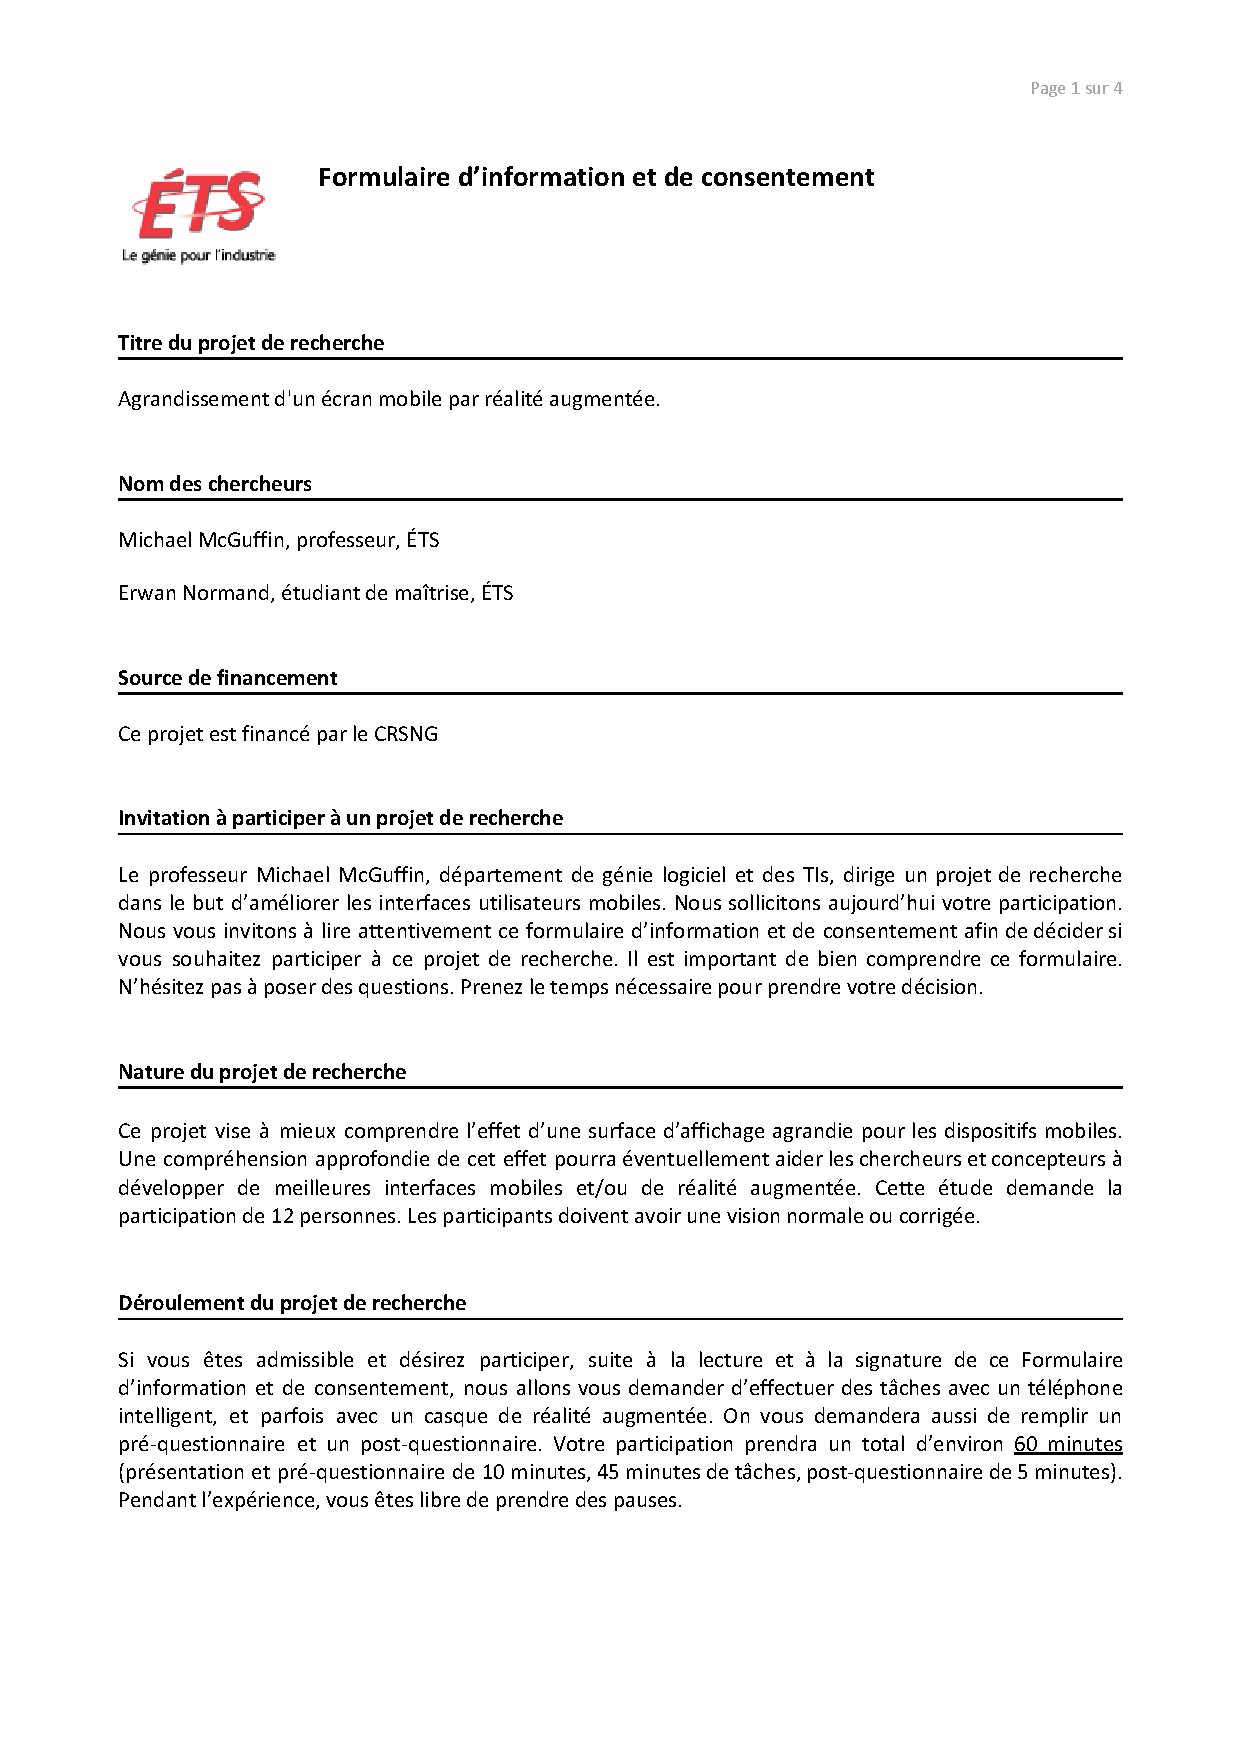
\includegraphics[page=1, scale=0.75, trim={0 0.5cm 0 2.5cm}, clip]{content/9_experiment_forms_1.pdf}
\includepdf[pages=2-]{content/9_experiment_forms_1.pdf}
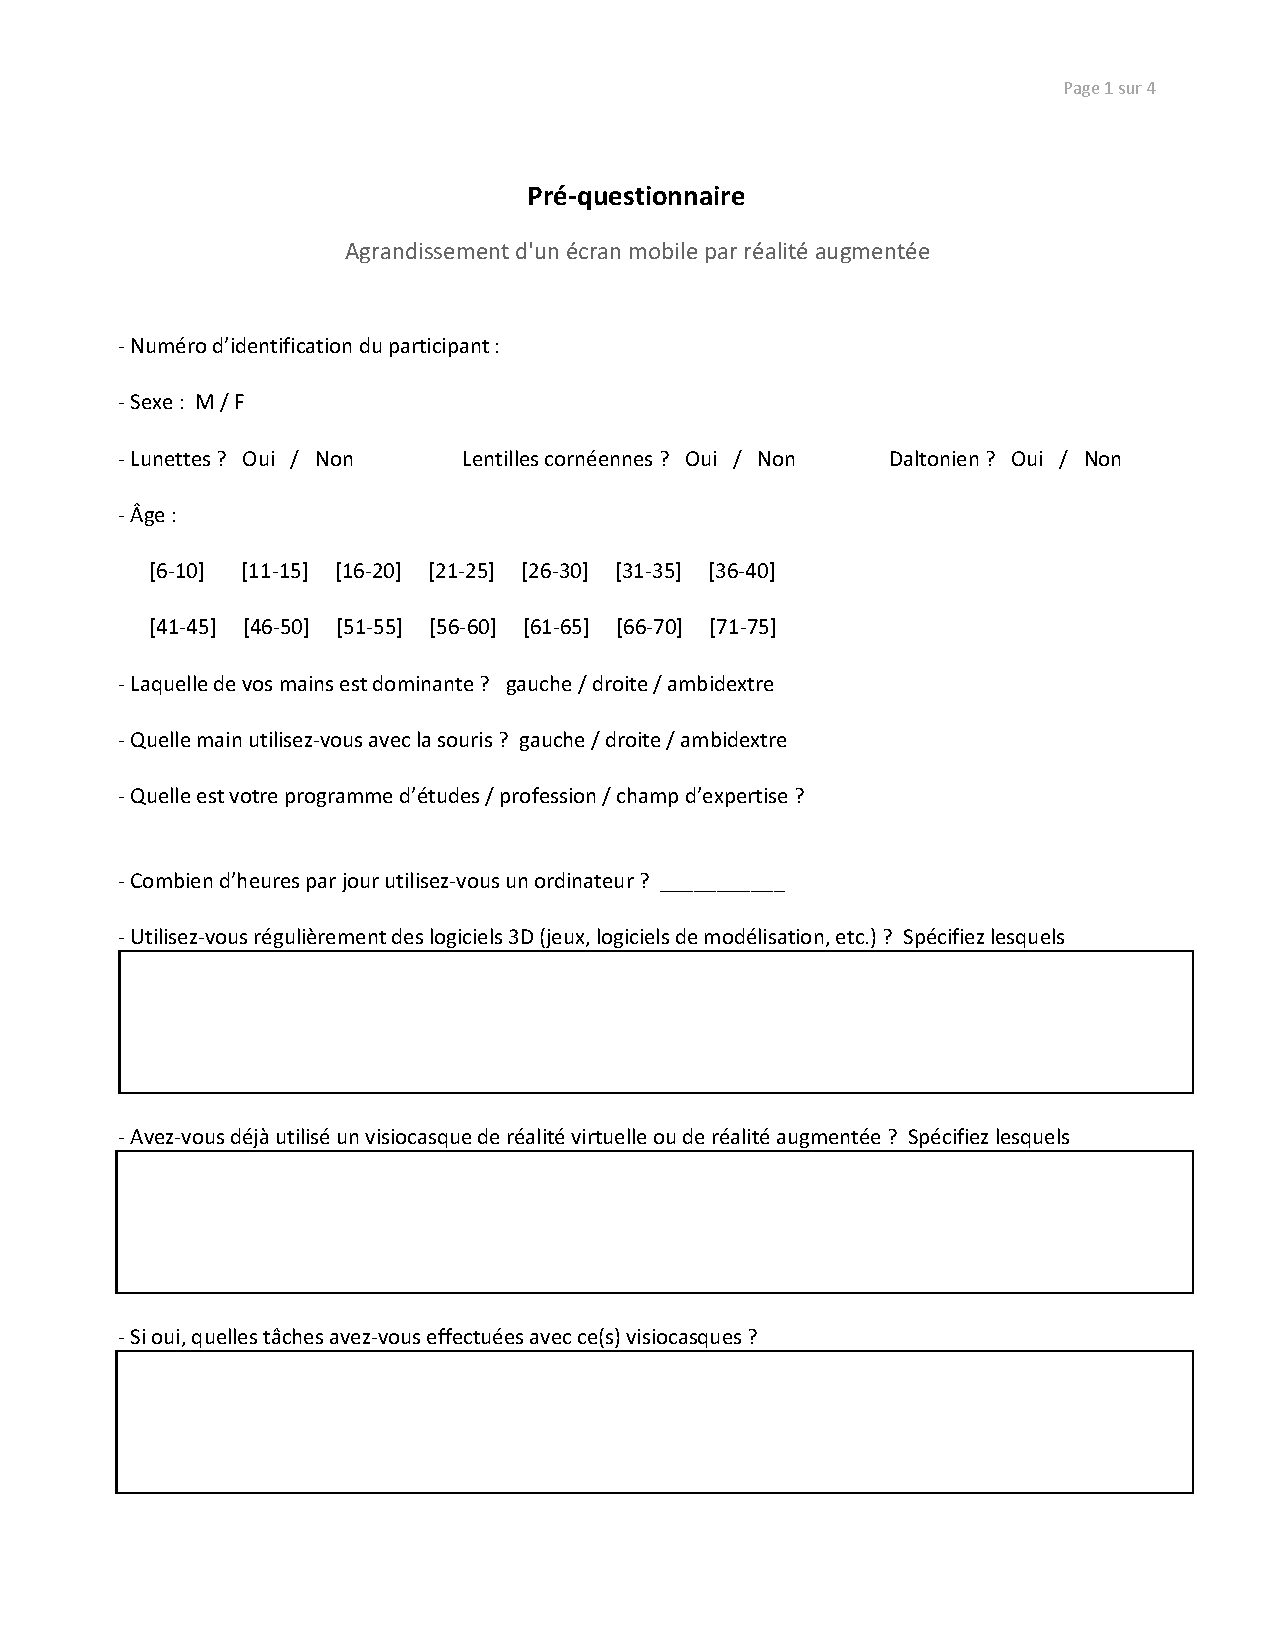
\includepdf[pages=-,]{content/9_experiment_forms_2.pdf}
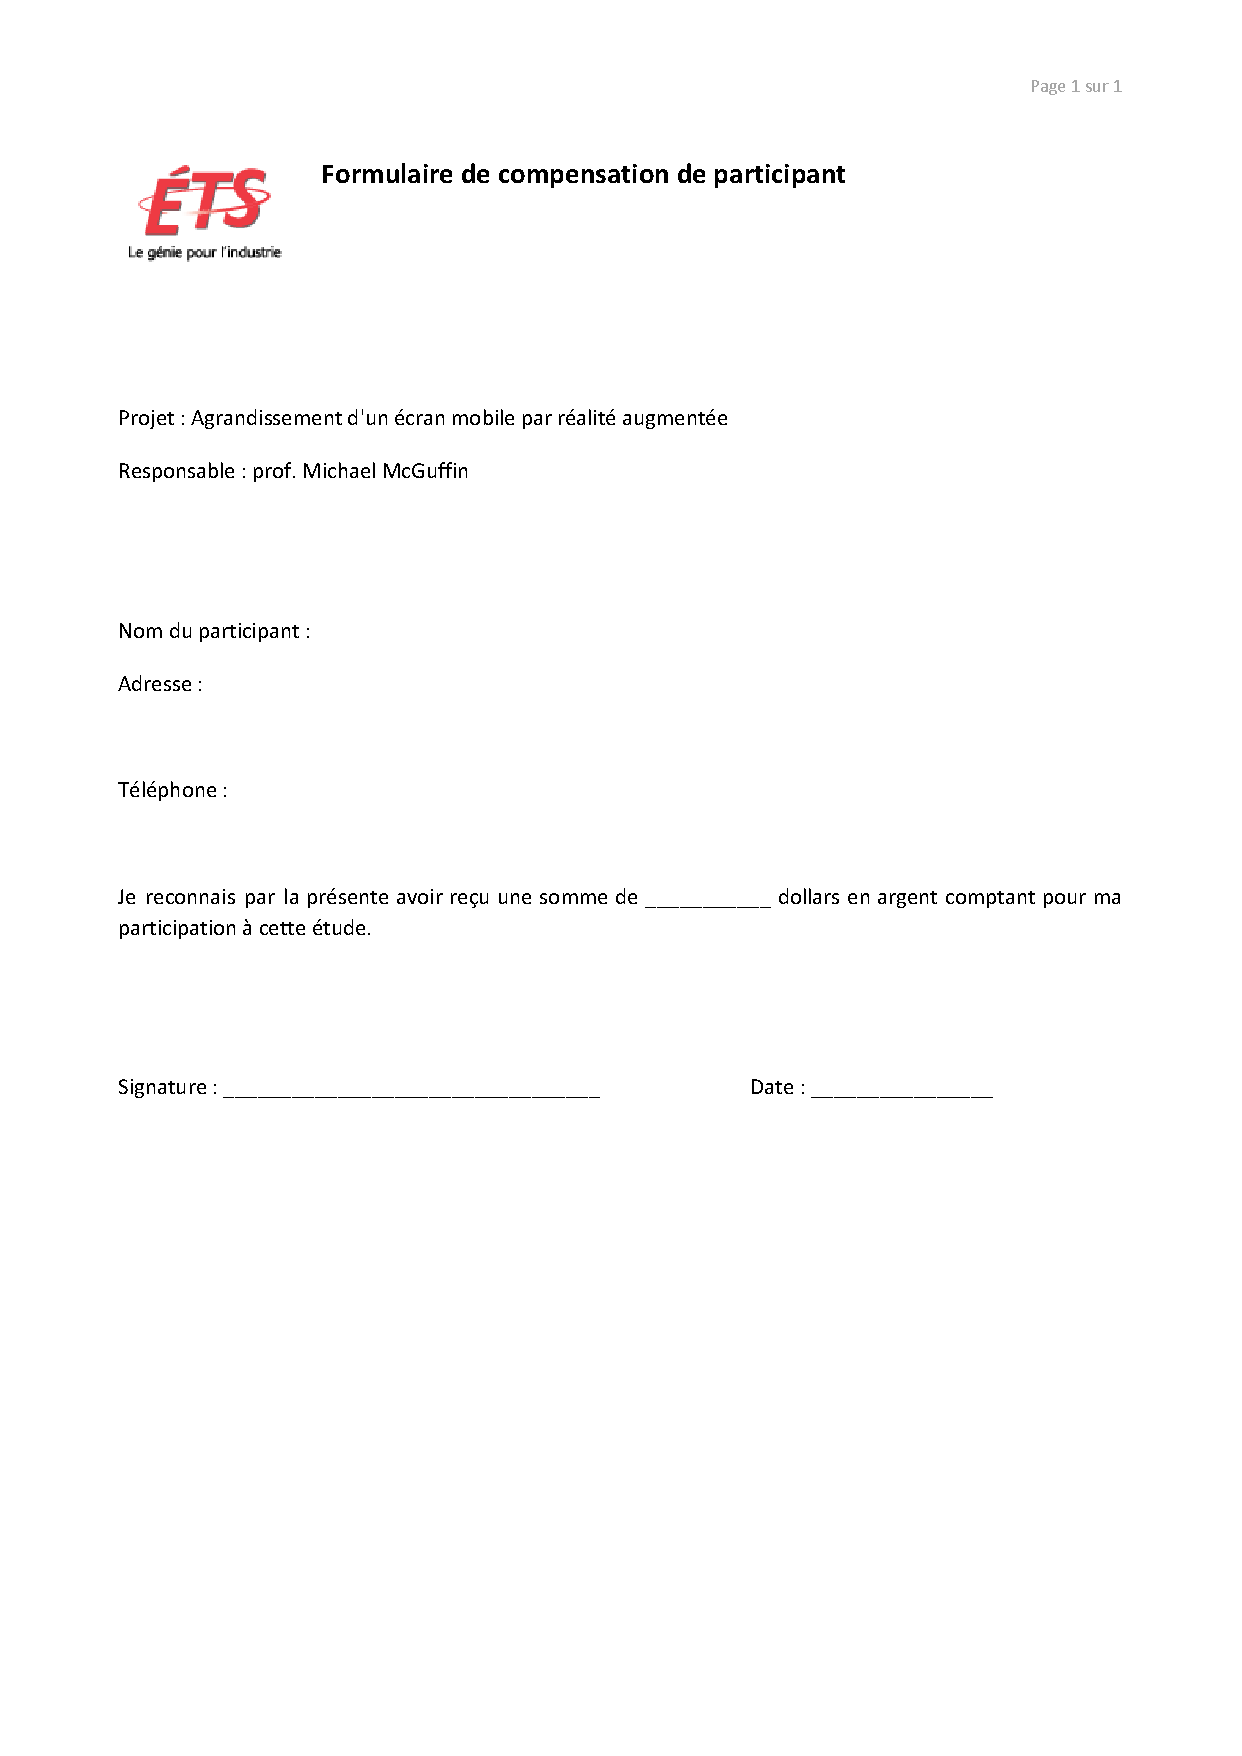
\includepdf[pages=-,]{content/9_experiment_forms_3.pdf}
%\chapter{Analyse détaillée de l'expérience}
\label{appendix:experiment_analysis}

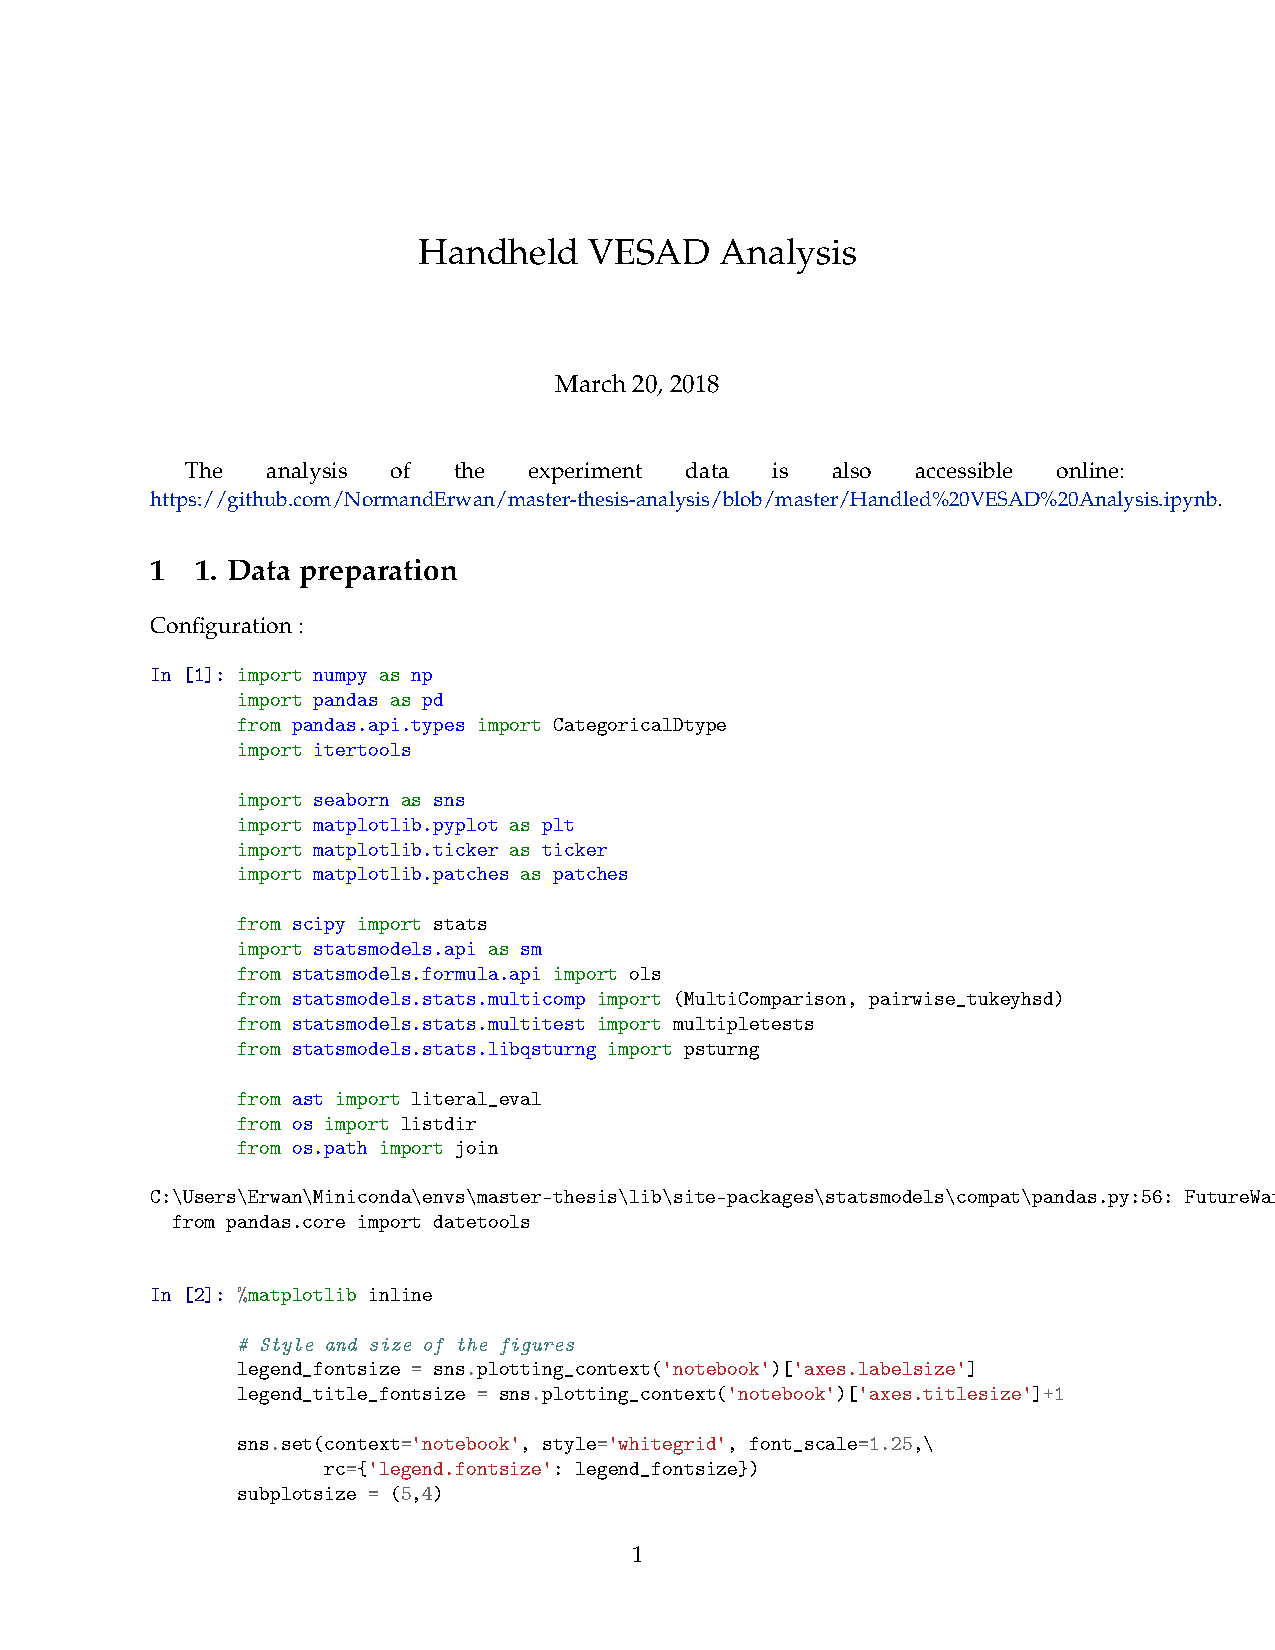
\includegraphics[page=1, scale=0.75, trim={0 0.5cm 0 3.5cm}, clip]{content/10_experiment_analysis.pdf}
\includepdf[pages=2-]{content/10_experiment_analysis.pdf}

\newpage
\begin{spacing}{1}
  \nocite{*}
  \bibliographystyle{bibETS}
  \addcontentsline{toc}{chapter}{BIBLIOGRAPHIE}
  \bibliography{bibliography/thesis}
\end{spacing}

\end{document}